\cotefile{142}
\scanpage{26}
\mspage{7}
\figure{
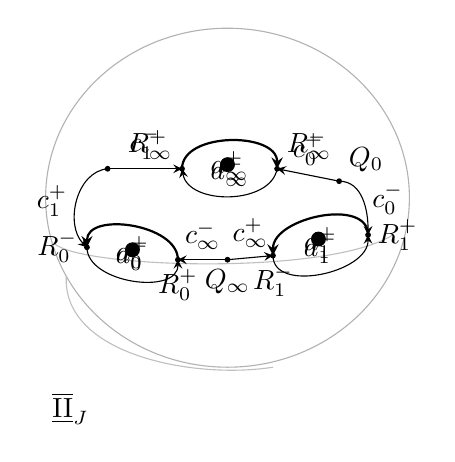
\begin{tikzpicture}[x=1.05cm,y=1.05cm,>=stealth]
\draw[gray!60] (0,.65) ellipse (2.2 and 2.05);
\draw[gray!50] (-2.1,.1) .. controls (-1.8,-.2) and (1.2,-.3) .. (2,.2);
\draw[gray!50] (-1.95,-.3) .. controls (-2,-1.25) and (-.4,-1.55) .. (.55,-1.4);
\coordinate (A) at (-.55,1);\coordinate (B) at (.6,1);
\coordinate (C) at (-1.7,.05);\coordinate (D) at (-.6,-.1);
\coordinate (E) at (.55,-.05);\coordinate (F) at (1.7,.2);
\coordinate (U) at (-1.45,1);\coordinate (V) at (1.35,.85);\coordinate (W) at (0,-.1);
\foreach \p in {A,B,C,D,E,F,U,V,W}{\fill (\p) circle (.035);}
\fill (0,1.05) circle (.09);\fill (-1.15,.02) circle (.09);\fill (1.1,.15) circle (.09);
\draw[->,thick] (A) to[out=90,in=90] node[below] {$a_\infty^+$} (B);
\draw[->] (B) to[out=260,in=280] node[above] {$a_\infty^-$} (A);
\draw[->,thick] (D) to[out=90,in=90] node[below] {$a_0^+$} (C);
\draw[->] (C) to[out=270,in=270] node[above] {$a_0^-$} (D);
\draw[->,thick] (F) to[out=90,in=90] node[below] {$a_1^+$} (E);
\draw[->] (E) to[out=270,in=270] node[above] {$a_1^-$} (F);
\draw[->] (U) to[out=185,in=135] node[left] {$c_1^+$} (C);
\draw[->] (U)--node[above] {$c_1^-$}(A);
\draw[->] (V)--node[above] {$c_0^+$}(B);
\draw[->] (V) to[out=0,in=90] node[right] {$c_0^-$}(F);
\draw[->] (W)--node[above] {$c_\infty^-$}(D);
\draw[->] (W)--node[above] {$c_\infty^+$}(E);
\node[above left] at(A){$R_\infty^+$};\node[above right] at(B){$R_\infty^-$};
\node[left] at(C){$R_0^-$};\node[below] at(D){$R_0^+$};
\node[below] at(E){$R_1^-$};\node[right] at(F){$R_1^+$};
\node[above right] at(V){$Q_0$};\node[below] at(W){$Q_\infty$};
\node at(-1.9,-1.9){$\overline{\underline{\mathrm{II}}}_J$};
\end{tikzpicture}
}
On rajoute les sommets $Q_i$ $(i\in J)$ et les arcs
\diagram{\begin{tikzcd}[ampersand replacement=\&]Q_i\arrow[r,"c_i^\omega"]\&R_{\omega'i}^{\omega'}\end{tikzcd}}
permutés \deleted{de façon simple transitivement} par $G_J$. On a maintenant
\[
(13)\qquad b_i^\omega=c_i^\omega(c_i^{\omega'})^{-1}
\]
(donc les $b_i^\omega$ deviennent inutiles comme générateurs d'un groupoïde). \inserted{Dans} Les relations \inserted{$(2)$} \deleted{deviennent} la partie $(a)$ devient automatique, pour écrire commodément la partie $(b)$, on introduit les
\[
(14)\qquad\widetilde a_i^\omega=
\deleted{(\unsure{c_{\omega i}^{\omega}})^{-1}a_i^{\unsure{\omega}}\unsure{c_{\omega'i}^{\omega'}}}
\inserted{(c_{\omega i}^\omega)^{-1}a_i^\omega c_{\omega'i}^{\omega'}}
:\quad Q_{\omega'i}\longrightarrow Q_{\omega i}
\]
\diagram{
\begin{tikzcd}[ampersand replacement=\&,column sep=small,row sep=large]
Q_{\omega i}\&R_i^{\omega'}\arrow[l,"(c_{\omega i}^{\omega})^{-1}"']\arrow[r,dashed,bend right=28,"a_i^{\omega'}"']\&R_i^\omega\arrow[l,bend right=45,"a_i^\omega"']\&Q_{\omega'i}\arrow[l,"c_{\omega'i}^{\omega'}"]\\
\deleted{\unsure{Q_{\omega i}}}\arrow[r,"\deleted{\unsure{c_{\omega i}^{\omega}}}"]\&\deleted{\unsure{R_i^\omega}}\arrow[r,bend right=45,"\deleted{a_i^{\omega'}}"']\&\deleted{\unsure{R_i^{\omega'}}}\arrow[r,"\deleted{(c_{\omega'i}^{\omega'})^{-1}}"']\&\deleted{\unsure{Q_{\omega'i}}}
\end{tikzcd}}
\margin{\figure{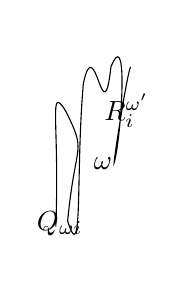
\begin{tikzpicture}[x=.5cm,y=.7cm]
\draw (0,0) .. controls (.1,1.9) and (-.2,2.6) .. (.25,2.1) .. controls (.8,1.3) and (.5,1.6) .. (.3,.1);
\draw (.3,.1) .. controls (.7,-.8) and (.5,1) .. (.7,2.6) .. controls (1,3.6) and (1.2,1.6) .. (1.4,2.9) .. controls (1.8,3.6) and (1.7,2.1) .. (1.55,1.4) .. controls (1.3,.4) and (1.8,2.8) .. (1.9,2.9);
\node at(.1,.05){$\unsure{Q_{\omega i}}$};\node at(1.2,1.15){$\omega$};\node at(1.8,2.1){$\unsure{R_i^{\omega'}}$};
\end{tikzpicture}}}
qui sont également permutés de façon simpl. transitive sous $G_J$, et on a
\[
(15)\qquad\tau(\widetilde a_i^\omega)=(\widetilde a_i^{\omega'})^{-1}
\]
La relation $(2b)$ devient
\[
(16)\qquad\widetilde a_{\omega^2i}^\omega\widetilde a_{\omega i}^\omega\widetilde a_i^\omega=1
\]
(deux relations ess\textsuperscript{t.} distinctes qui sont permutées par $\tau$)

Pour repérer les \inserted{$\pi(Q_i)=$} $\pi_1(\Sigma_J(\mathbb C),Q_i)$ de façon commode on utilise les
\diagram{
\begin{tikzcd}[ampersand replacement=\&,column sep=large,row sep=large]
(17)\quad\psi_i^\omega:\ \deleted{\unsure{Q}}\Pi_{0,3}\arrow[rr,"\sim"]\arrow[dr,"\varphi_{\omega'i}^{\omega'}"',"\sim"]\&\&\pi(Q_i)\\
\&\pi(R_{\omega'i}^{\omega'})\arrow[ur,"(c_i^\omega)^{-1}"',"\sim"]\&
\end{tikzcd}}
\margin{\uline{NB}\quad$\tau\psi_i^\omega(g)=\psi_i^{\omega'}(\tau_\infty g)$}
on aura
\[
(18)\qquad\psi_i^\omega(g)=\psi_i^{\omega'}(\sigma_\infty(g))
\]
\[
(19)\qquad\begin{aligned}
\widetilde a_i^{\omega\deleted{\unsure{'}}}(\psi_{\omega'i}^{\omega'}(g))
&=\psi_{\omega\deleted{\unsure{'}}i}^{\omega\deleted{\unsure{'}}}(\varepsilon_0(g))
=\psi_{\omega\deleted{\unsure{'}}i}^{\omega'}(\overbrace{\sigma_\infty\varepsilon_0}^{\deleted{\unsure{\xi}}\tau_\infty(\rho)}(g))\\
\boxed{\widetilde a_i^\omega(\psi_{\omega'i}^{\omega}(g))
=\psi_{\omega\deleted{\unsure{'}}i}^{\omega\deleted{\unsure{'}}}(\overbrace{\varepsilon_0\sigma_\infty}^{\rho^{-1}}(g))}
=\psi_{\omega i}^{\omega'}(\sigma_\infty\varepsilon_0\sigma_\infty(g))
\end{aligned}
\]
\margin{25}

\scanpage{27}
\mspage{8}
On prend un autom. \inserted{$u$} du groupoïde $\widehat{\overline{\underline{\mathrm{II}}}}_J$ qui \inserted{commute à $G_J$ et qui} fixe les sommets, et qui comme plus haut laisse stables les sous-groupoïdes $\widehat{\overline{\underline{\mathrm{II}}}}_{J,i}$ $(i\in J)$, \deleted{les groupoïdes} $\overline{\underline{\mathrm{II}}}_{J,i}$ engendré par les \inserted{2} sommets $R_i^\omega$ $(\omega\in\uline{\omega})$ et les deux flèches $a_i^\omega$ $(\omega\in\uline{\omega})$.
\deleted{Alors} L'endom. $u$ est connu quand on connaît les $u(a_i^\omega)$, qui sont de la forme
\[
(20)\qquad u(a_i^\omega)=a_i^\omega\varphi_i^\omega\bigl(\underbrace{l_0^\gamma}\bigr)
\qquad\begin{array}{l}\gamma=\frac{p-1}{2}\in\widehat{\mathbb Z}\\p\in\widehat{\mathbb Z}^{*}\end{array}
\]
\margin{NB: $\lambda\in\widehat\Pi_{0,3}$, pas la peine d'exiger de prime abord que $\lambda$ de la forme $l_0^\gamma\ldots$}
\uline{et} les
\[
(21)\qquad u(c_i^\omega)=\varphi_{\omega'i}^{\omega'}(\eta)c_i^\omega=c_i^\omega\psi_i^\omega(\eta)
\qquad\eta\in\widehat\Pi_{0,3}\quad\text{indépendant de }i,\omega
\]
On aura alors (comparer $(11)$)
\[
(22)\qquad u(b_i^\omega)=b_i^\omega\varphi_{\omega i}^\omega(\beta)\qquad\text{avec}
\]
\[
(23)\qquad\beta=\sigma_\infty(\eta)\eta^{-1}
\]
\margin{NB devient plus joli si $\eta$ est remplacé par son $\sigma_\infty\eta$, ou $\beta$ par $\beta^{-1}$}
Les relations à satisfaire \deleted{\unsure{sont}} alors déjà écrites en \inserted{$p$ (ou $\gamma$) et} $\beta$, \deleted{\unsure{la}} dans $(12)$ --- mais la première relation $\beta\sigma_\infty(\beta)=1$ conséquence de $(23)$, il reste la deuxième qui s'écrit donc
\margin{\uline{NB} Si $u$ remplacé par $u'=\tau(u)$, alors $\eta$ est remplacé par $\eta'=\tau_\infty(\eta)$, $\beta$ par $\tau_\infty(\beta)$, mais $\lambda$ par $\varepsilon_0^{-1}(\tau_\infty(\lambda^{-1}))$.}
\[
(24)\qquad\deleted{(l_1^{-\gamma}\sigma_\infty(\eta)\eta^{-1}}
\quad\alpha\rho^{-1}(\alpha)\rho^{-2}(\alpha)=1
\qquad\text{avec}\quad\alpha=\underbrace{l_1^\gamma}_{\sigma_\infty(\lambda)}\underbrace{\sigma_\infty(\eta)\eta^{-1}}_\beta.
\]
On aura ici
\[
(25)\qquad
u(\widetilde a_i^\omega)=\psi_{\omega\deleted{\unsure{'}}i}^{\omega\deleted{\unsure{'}}}\bigl(\underbrace{\eta^{-1}l_0^\gamma\varepsilon_0(\eta)}_{\widetilde\alpha=\eta^{-1}\varepsilon_0(\lambda\eta)}\bigr)\widetilde a_i^\omega
=\widetilde a_i^\omega\psi_{\omega'i}^{\omega'}\bigl(\underbrace{\varepsilon_0^{-1}(\eta^{-1})l_0^\gamma\eta}_{\varepsilon_0^{-1}(\widetilde\alpha)}\bigr)
\]
\inserted{valable quel que soit $\lambda$}
\margin{$\widetilde\alpha=\eta^{-1}l_0^\gamma\varepsilon_0(\eta)$}
et
\[
(25\text{ bis})\quad\deleted{\unsure{\alpha=}}\quad\alpha=\rho\bigl(\eta\widetilde\alpha\rho^{-1}(\eta)^{-1}\bigr)
\]
\margin{valable pour $\lambda$ quelconque, pas néc. de la forme $l_0^\gamma$.}
\deleted{car} dans l'équation $(24)$ en $\alpha$ (invariante par substitutions $\alpha\mapsto\rho^{-1}(\alpha)$ (ou $\alpha\mapsto\rho\alpha=\rho^{-2}(\alpha)$) et $\alpha\mapsto x\alpha\rho^{-1}(x)^{-1}$,
\margin{26}

\scanpage{28}
\mspage{9}
équivaut à l'équation \deleted{identique} \deleted{correspondante} \inserted{analogue} en $\widetilde\alpha$
\[
(26)\qquad\widetilde\alpha\rho^{-1}(\widetilde\alpha)\rho^{-2}(\widetilde\alpha)=1,
\qquad\boxed{(27)\quad\widetilde\alpha=\eta^{-1}l_0^\gamma\varepsilon_0(\eta)}
\]
\deleted{$\unsure{\varepsilon}$}
Considérons maintenant le groupoïde \inserted{$\overline{\underline{\mathrm{III}}}_J$} induit par le groupoïde précédent \inserted{$\overline{\underline{\mathrm{II}}}_J$} sur l'ens des trois sommets $Q_i$, c'est aussi le groupoïde engendré par le graphe à trois sommets $Q_i$ $(i\in J)$ et six arcs orientés $\widetilde a_i^\omega$ et leurs opposés, avec les seules relations $(16)$ (ens de 6 relations stable par $G_J$, et se réduisant en fait à deux relations effectives\ldots).
\figure{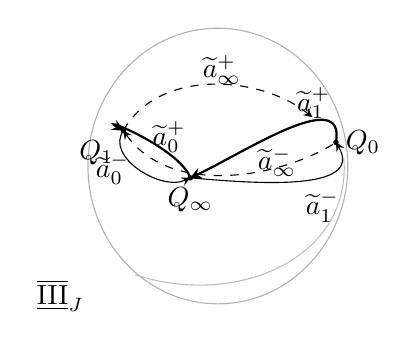
\begin{tikzpicture}[x=1cm,y=1cm,>=stealth]
\draw[gray!60] (0,.1) ellipse (1.65 and 1.75);
\draw[gray!50] (-1.05,-1.28) .. controls (.2,-1.7) and (1.7,-1.1) .. (1.6,.2);
\coordinate (A) at (-1.2,.55);\coordinate (B) at (-.35,-.05);\coordinate (C) at (1.5,.4);
\foreach \p in {A,B,C}{\fill(\p) circle(.035);}
\draw[->,thick] (B) to[out=110,in=150] node[right] {$\widetilde a_0^+$} (A);
\draw[->] (A) to[out=235,in=205] node[left] {$\widetilde a_0^-$} (B);
\draw[->,thick] (C) to[out=80,in=25] node[above right] {$\widetilde a_1^+$} (B);
\draw[->] (B) to[out=-5,in=300] node[below right] {$\widetilde a_1^-$} (C);
\draw[->,dashed] (A) .. controls (-.75,1.35) and (.55,1.25) .. (1.2,.72);
\node at(.05,1.32){$\widetilde a_\infty^+$};
\draw[<-,dashed] (A) .. controls (-.6,-.3) and (.8,-.05) .. (C);
\node at(.75,.15){$\widetilde a_\infty^-$};
\node[below left] at(A){$Q_1$};\node[below] at(B){$Q_\infty$};\node[right] at(C){$Q_0$};
\node at(-2,-1.55){$\overline{\underline{\mathrm{III}}}_J$};
\end{tikzpicture}}
Le groupe $\{1,\tau\}$ y opère dans le graphe avec relations, par
\[
(27)\qquad\tau Q_i=Q_i,\quad\tau\widetilde a_i^\omega=(\widetilde a_i^{\omega'})^{-1}
\]
La donnée d'un \deleted{autom.} \inserted{endom.} du groupoïde $\overline{\underline{\mathrm{III}}}_J$, fixant les sommets et commutant à $G_J$, équivaut à celle d'un $\widetilde\alpha\in\widehat\Pi_{0,3}$, \deleted{$\unsure{\in\widehat{\mathbb Z}}$}, satisfaisant \deleted{\unsure{l'équation rel.}} $(26)$. On aura, en introduisant
\[
(28)\qquad\widetilde\lambda_i^\omega=\widetilde a_i^{\omega'}\widetilde a_i^\omega\in\deleted{\unsure{Q_{\omega'i}}}\inserted{\pi(Q_{\omega'i})}
\]
(comparer à la définition dans le groupoïde $\overline{\underline{\mathrm{II}}}_J$ ! $\lambda_i^\omega=a_i^{\omega'}a_i^\omega$)
\diagram{\begin{tikzcd}[ampersand replacement=\&,column sep=small]
Q_{\omega i}\arrow[rrr,bend right=45,"\widetilde a_i^{\omega'}"']\&R_i^{\omega'}\arrow[l,dashed,no head]\arrow[r,dashed,bend right=40]\&R_i^\omega\arrow[l,dashed,bend right=40,"a_i^\omega"']\arrow[r,dashed,no head]\&Q_{\omega'i}\arrow[lll,bend right=45,"\widetilde a_i^{\omega\deleted{\unsure{'}}}"']
\end{tikzcd}}
\margin{\deleted{il semblerait raisonnable de changer les notations $\widetilde a_i^\omega$ devenant $\widetilde a_i^{\omega'}$.}\quad $*$ \unsure{tenir|obtenir}, \unsure{une définition des} $\psi_i^\alpha$ \unsure{qui} \unsure{donne} dans $(29)$ \unsure{ainsi le}. cf. voir plus bas}
\[
(29)\qquad u(\widetilde\lambda_i^\omega)=\overset{*}{\psi_{\omega'i}^{\omega'}}(\widetilde\alpha\varepsilon_0(\widetilde\alpha))\widetilde\lambda_i^\omega
=\psi_{\omega'i}^{\omega'}(\widetilde\alpha\varepsilon_0(\widetilde\alpha)l_0)
\]
Dans le cas où $\widetilde\alpha$ provient de $\eta,\gamma$ par $(27)$, on aura
\[
(30)\qquad\widetilde\alpha\varepsilon_0(\widetilde\alpha)l_0=\eta^{-1}l_0^p\eta\qquad(p=2\gamma+1)\ ;
\]
\margin{27}

\scanpage{29}
\mspage{10}
\margin{\uline{NB} Ce sous-groupoïde $\overline{\underline{\mathrm{III}}}_{J,i}$ (de groupe fondamental $\widehat{\mathbb Z}$) engendré par les sommets $Q_j$ $(j\in J\setminus\{i\})$ et les deux $\unsure{\widetilde a_i^\omega}$ orientés qui les joignent, \uuline{n'est \deleted{\unsure{donc}} pas} (!) stable \uline{par $u$} !}
en d'autres termes faisons opérer $u$ sur $\pi(Q_{\omega'i})$, identifié à $\widehat\Pi_{0,3}$ via $\psi_{\omega'i}^{\omega'}$, $\widetilde\lambda_i^\omega$ identifié à $l_0$, on trouve que $u(l_0)$ est conjugué de $l_0^p$, \deleted{avec} la conjugaison étant effectuée par $\eta^{-1}$ (par la formule $(30)$).

Le passage de $u$ à $\tau(u)$ s'exprime par
\deleted{J'en prends maintenant les points $P_\omega^{\unsure{\omega}}$ $(\omega\in\uline{\omega})$}
le passage de $\widetilde\alpha$ à
\[
(31)\qquad\widetilde\alpha'=\varepsilon_0\tau_\infty(\widetilde\alpha^{-1})
=\underbrace{\rho^{-1}\widetilde\sigma_\infty}_{\widetilde\sigma_0}(\widetilde\alpha^{-1})
\]
\margin{où $\widetilde\sigma_\infty=\sigma_\infty\tau_\infty=\tau_\infty\sigma_\infty$ est dans l'image de l'hom canonique
\diagram{\begin{tikzcd}[ampersand replacement=\&]\widetilde G_3\arrow[r]\&\widetilde\Pi_{0,3}\end{tikzcd}}
$\simeq$\quad\deleted{\unsure{du}\ $\widetilde G_3$}
stabilisateur de $P_+$ dans $G_3\times\{1,\tau\}$}
\[
\widetilde\sigma_i(l_i)=l_i^{-1}
\]
\[
\widetilde\sigma_i(l_j)=l_k^{-1}\quad\text{si }\{0,1,\infty\}=\{i,j,k\}
\]
\uline{NB} le groupe $\widetilde G_3$ opère sur $\Pi_{0,3}$ et contient \deleted{$\unsure{\xi}$} \deleted{dont il} $\{1,\rho^{-1},\rho_{\unsure{\mathrm{II}}}^{-2}\}$ comme ss-groupe \inserted{$\widetilde G_3^+$} d'indice 2, \deleted{\unsure{dont $\widetilde G_3$ conjugue $\rho$}} $\widetilde G_3/\widetilde G_3^+$ opère sur $\widetilde G_3^+$ en échangeant $\rho$ et $\rho^{-1}$, il s'ensuit que $\widetilde G_3$ opère sur $V$ ens des solutions $x$ de l'équation
\[
x\rho^{-1}(x)\rho^{-2}(x)=1
\]
par
\[
(32)\qquad\Theta_g x=g.x^{\operatorname{sg}(g)}
\]
et on a ici
\[
(33)\qquad\widetilde\alpha'=\Theta_{\widetilde\sigma_0}(\widetilde\alpha)
\]
\margin{28}

\scanpage{30}
\margin{29}
\mspage{11}
\margin{\uline{NB} les flèches $\widetilde a_i^\omega$ sont en fait superflues, cf $(37)$ et commentaires p. 19.}
\figure{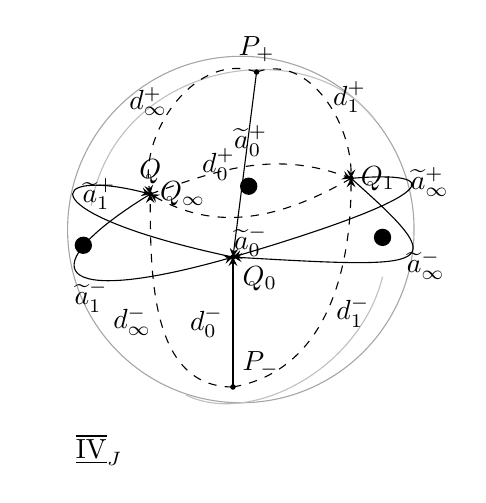
\begin{tikzpicture}[x=1cm,y=1cm,>=stealth]
\draw[gray!70] (0,0) ellipse (2.2 and 2.2);
\draw[gray!50] (-1.9,.3) .. controls (-1.6,2.1) and (.8,2.55) .. (1.7,1.4);
\draw[gray!50] (-.7,-2.1) .. controls (.1,-2.5) and (1.5,-1.8) .. (1.8,-.6);
\coordinate(P) at(.2,2);\coordinate(M) at(-.1,-2);\coordinate(A) at(-1.15,.45);\coordinate(B) at(1.4,.65);\coordinate(C) at(-.1,-.35);
\foreach \p in {P,M,A,B,C}{\fill (\p) circle(.035);}
\fill (-2,-.2) circle(.11);\fill(.1,.55) circle(.11);\fill(1.8,-.1) circle(.11);
\draw[->,dashed] (P) to[out=160,in=100] node[left]{$d_\infty^+$}(A);
\draw[->] (P)--node[left]{$d_0^+$}(C);
\draw[->,dashed] (P) to[out=20,in=90] node[right]{$d_1^+$}(B);
\draw[->,dashed] (M) to[out=180,in=270] node[left]{$d_\infty^-$}(A);
\draw[->] (M)--node[left]{$d_0^-$}(C);
\draw[->,dashed] (M) to[out=10,in=270] node[right]{$d_1^-$}(B);
\draw[->,dashed] (A) to[out=20,in=160] node[above]{$\widetilde a_0^+$}(B);
\draw[->,dashed] (B) to[out=210,in=330] node[below]{$\widetilde a_0^-$}(A);
\draw[->] (C) .. controls (-2.7,.2) and (-2.5,.8) .. (A);
\node at(-1.8,.45){$\widetilde a_1^+$};
\draw[->] (A) .. controls (-2.7,-.5) and (-2.4,-1) .. (C);
\node at(-1.9,-.85){$\widetilde a_1^-$};
\draw[->] (B) .. controls (2.6,.75) and (2.6,.45) .. (C);
\node at(2.4,.6){$\widetilde a_\infty^+$};
\draw[->] (B) .. controls (2.7,-.5) and (2.5,-.5) .. (C);
\node at(2.35,-.45){$\widetilde a_\infty^-$};
\node[above] at(P){$P_+$};\node[above right] at(M){$P_-$};
\node[right] at(A){$Q_\infty$};\node[right] at(B){$Q_1$};\node[below right] at(C){$Q_0$};
\node[above] at(A){$\deleted{\unsure{Q}}$};\node at(-1.8,-2.8){$\overline{\underline{\mathrm{IV}}}_J$};
\end{tikzpicture}}
On rajoute les \inserted{deux} sommets $P_i^\omega$ $(\omega\in\uline{\omega})$, et les flèches
\diagram{\begin{tikzcd}[ampersand replacement=\&]d_i^\omega:\quad P_\infty^\omega\arrow[r]\&Q_i\end{tikzcd}}
permutés transitivement par $G_J$, avec
\[
(34)\qquad\tau(P_{\unsure{\infty|i}}^\omega)=P_{\unsure{\infty|i}}^{\omega'},\qquad\tau(d_i^\omega)=d_i^{\omega'}
\]
Le groupoïde $\overline{\underline{\mathrm{III}}}_J$ est équivalent au groupoïde $\overline{\underline{\mathrm{IV}}}_J$ \inserted{défini par le graphe ayant} \deleted{sur} les sommets $Q_i$ $(i\in\omega)$ et $P_\infty^\omega$ $(\omega\in\uline{\omega})$, les arcs $\widetilde a_i^\omega$ et $d_i^\omega$ et les \inserted{arcs} opposés, et les six relations
\[
(35)\qquad(d_{\omega'i}^\omega)^{-1}\widetilde a_{\omega i}^{\omega}d_i^\omega=1
\]
(qui impliquent d'ailleurs les relations constitutives $(16)$ pour $\overline{\underline{\mathrm{III}}}_J$). La donnée d'un endomorphisme de $\overline{\underline{\mathrm{IV}}}_J$ qui fixe les \deleted{pts} sommets (pour simplifier --- il faudra regarder aussi ceux qui permutent les sommets \inserted{$P_\omega$} en fixant les $Q_i$), \deleted{équivaut à} et qui commute à $G_J$, équivaut à la donnée des
\[
(36)\quad\left\{\begin{aligned}
u(\widetilde a_i^\omega)&=\psi_{\omega i}^\omega(\widetilde\alpha)\widetilde a_i^\omega
&\widetilde\alpha&\in\widehat\Pi_{0,3}\quad\text{(indép. de }i,\omega\text{)}\\
u(d_i^\omega)&=\psi_i^\omega(\zeta)d_i^\omega\quad\bigl(=d_i^\omega\widetilde\psi_i^\omega(\zeta)\bigr)
&\zeta&\in\widehat\Pi_{0,3}\quad\cdots
\end{aligned}\right.
\]
\deleted{\unsure{u}}
de $\widetilde\alpha,\zeta\in\widehat\Pi_{0,3}$, avec la relation déduite de $(35)$, on trouve les équations
\[
(37)\qquad\widetilde\alpha=\zeta.\rho^{-1}(\zeta^{-1}),
\]
i.e. $\widetilde\alpha$ est connu quand on connaît $\zeta\in\widehat\Pi_{0,3}$.
\margin{il n'y a donc pas de condition \unsure{+} sur $\zeta$ ici.}

\scanpage{31}
\mspage{12}
qui implique bien sûr (26).

\margin{revenant avant l'introduction de $u$}
Je \deleted{vais} considère les isomorphismes
\diagram{\begin{tikzcd}[ampersand replacement=\&,column sep=large,row sep=large]
\Pi_{0,3}\arrow[r,"\widetilde\psi_i^\omega"]\arrow[dr,"\psi_i^\omega"']\&\pi(P^\omega)\\
\&\pi(Q_i)\arrow[u,"(d_i^\omega)^{-1}"']
\end{tikzcd}}\quad(38)
\margin{\uline{NB} le passage de $u$ à $\tau(u)$ s'exprime par
$\zeta\mapsto\sigma_\infty\tau_\infty(\zeta)=\widetilde\sigma_\infty(\zeta)$}
\margin{\deleted{\unsure{Changement} \unsure{de base} \unsure{au départ} de l'iso $\Pi_{0,3}\simeq\Pi_{0,3}$} pour une \unsure{compatib.}}

de sorte que les relations (35) et (19) donnent
\[
(39)\qquad \widetilde\psi_{\omega i}^\omega(g)=\widetilde\psi_i^\omega(\rho g)
\qquad\text{i.e.}\quad\widetilde\psi_{\omega i}=\widetilde\psi_i\circ\rho,
\]
\inserted{\figure{\begin{tikzpicture}\node[draw,ellipse] {$\rho^{-1}$?};\end{tikzpicture}}}
et j'introduis les chemins
\[
(40)\qquad\widetilde d_i^\omega:
\begin{tikzcd}[ampersand replacement=\&,column sep=large]
P_{\infty}^\omega\arrow[r,no head]\&P_{\infty}^{\omega'}
\end{tikzcd},\qquad
\widetilde d_i^\omega=(d_i^{\omega'})^{-1}d_i^\omega
\]
permutés de façon simplement transitive par $G_J$,
\deleted{de \illegible{1} et satisfaisant} satisfaisant
\[
(41)\qquad\tau(\widetilde d_i^\omega)=\widetilde d_i^{\omega'},\qquad
 d_i^\omega d_i^{\omega'}=1
\]
On \deleted{aura donc} \inserted{a} les relations
\[
(42)\qquad\widetilde d_i^\omega(\widetilde\psi_i^\omega(g))=
\widetilde\psi_i^{\omega'}(\sigma_\infty(g)).
\]
Revenant à l'\deleted{auto}morphisme $u$, on aura \deleted{automatiquement}
\[
(43)\qquad u(\widetilde d_i^\omega)=\widetilde\psi_i^{\omega'}(\unsure{\sigma_\infty|\tau_\infty}(\widetilde\beta))\widetilde d_i^\omega
=\widetilde d_i^\omega\widetilde\psi_i^\omega(\widetilde\beta)
\]
avec
\[
(44)\qquad\widetilde\beta=\zeta\sigma_\infty(\zeta)^{-1}.
\]
satisfaisant \inserted{donc} \deleted{\unsure{ainsi}} comme $\widetilde\beta$ doit, la relation
\[
(45)\qquad\widetilde\beta\sigma_\infty(\widetilde\beta)=1.
\]

Considérons maintenant le ss-groupoïde de
\margin{30}

\scanpage{33}
\mspage{14}
\figure{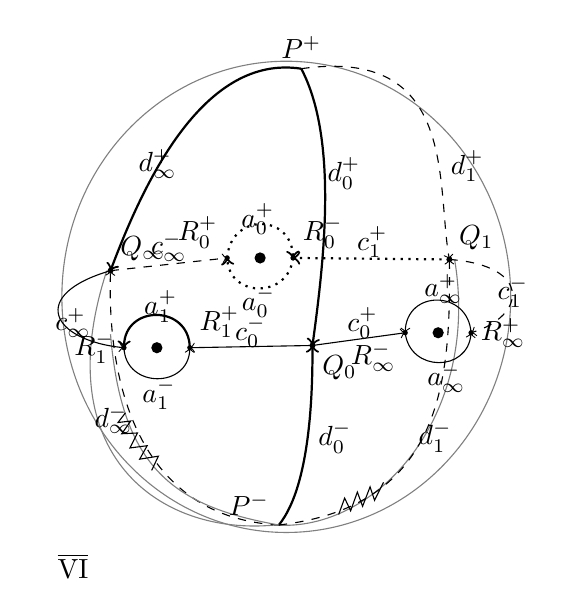
\begin{tikzpicture}[scale=.95]
\draw[gray] (0,0) ellipse (3 and 3.15);
\draw[gray] (-2.4,.35)..controls (-3.2,-2.1) and (-1.7,-3.2)..(-.15,-3.05);
\draw[gray] (2.25,.5)..controls (2.6,-1.6) and (1.2,-3.15)..(-.15,-3.05);
\coordinate (Pp) at (.2,3.05);\coordinate (Pm) at (-.1,-3.05);
\coordinate (Qi) at (-2.35,.35);\coordinate (Qz) at (.35,-.65);\coordinate (Qo) at (2.18,.5);
\draw[->,thick] (Pp)..controls (-1.1,3.25) and (-1.9,1.55)..(Qi);
\draw[->,thick] (Pp)..controls (.7,2.1) and (.5,.45)..(Qz);
\draw[dashed,->] (Pp)..controls (2.3,3.35) and (2,1.5)..(Qo);
\draw[dashed,->] (Pm)..controls (-1.95,-2.95) and (-2.4,-1.2)..(Qi);
\draw[->,thick] (Pm)..controls (.35,-2.5) and (.35,-1.1)..(Qz);
\draw[dashed,->] (Pm)..controls (2.1,-2.8) and (2.2,-1.1)..(Qo);
\draw[gray] (-2.35,-.5)..controls (-2.2,-2.3) and (-1.5,-2.8)..(-.1,-3.05);
\draw (-2.15,-1.55)--(-2.25,-1.68)--(-2.08,-1.66)--(-2.2,-1.83)--(-1.99,-1.82)--(-2.09,-2.02)--(-1.86,-1.99)--(-1.96,-2.17)--(-1.71,-2.13)--(-1.8,-2.32);
\draw (.7,-2.91)--(.78,-2.69)--(.86,-2.86)--(.95,-2.61)--(1.02,-2.8)--(1.12,-2.54)--(1.18,-2.72)--(1.3,-2.48);
\foreach \p in {Qi,Qz,Qo}{\fill (\p) circle (.04);}
\node[above] at (Pp) {$P^+$};\node[above left] at (Pm) {$P^-$};
\node[above right] at (Qi) {$Q_\infty$};\node[below right] at (Qz) {$Q_0$};\node[above right] at (Qo) {$Q_1$};
\node at (-1.72,1.78) {$d_\infty^+$};\node at (.77,1.65) {$d_0^+$};\node at (2.42,1.75) {$d_1^+$};
\node at (-2.31,-1.64) {$d_\infty^-$};\node at (.65,-1.88) {$d_0^-$};\node at (1.99,-1.87) {$d_1^-$};
\fill (-.35,.52) circle (.075);\fill (-1.73,-.68) circle (.075);\fill (2.03,-.48) circle (.075);
\coordinate (Rzp) at (-.79,.52);\coordinate (Rzm) at (.09,.52);
\coordinate (Rom) at (-2.17,-.68);\coordinate (Rop) at (-1.29,-.68);
\coordinate (Rim) at (1.59,-.48);\coordinate (Rip) at (2.47,-.48);
\draw[dotted,thick,->] (Rzp)..controls (-.75,1.12) and (.07,1.12)..(Rzm);
\draw[dotted,thick,->] (Rzm)..controls (.03,-.02) and (-.75,-.02)..(Rzp);
\draw[->,thick] (Rop)..controls (-1.3,-.1) and (-2.16,-.1)..(Rom);
\draw[->] (Rom)..controls (-2.15,-1.23) and (-1.3,-1.23)..(Rop);
\draw[->] (Rip)..controls (2.43,.1) and (1.6,.1)..(Rim);
\draw[->] (Rim)..controls (1.65,-1.01) and (2.43,-1.01)..(Rip);
\foreach \p in {Rzp,Rzm,Rom,Rop,Rim,Rip}{\fill (\p) circle (.035);}
\node[above left] at (Rzp) {$R_0^+$};\node[above right] at (Rzm) {$R_0^-$};
\node[left] at (Rom) {$R_1^-$};\node[above right] at (Rop) {$R_1^+$};
\node[below left] at (Rim) {$R_\infty^-$};\node[right] at (Rip) {$R_\infty^+$};
\node at (-.38,1.04) {$a_0^+$};\node at (-.37,-.07) {$a_0^-$};
\node at (-1.68,-.13) {$a_1^+$};\node at (-1.7,-1.3) {$a_1^-$};
\node at (2.1,.11) {$a_\infty^+$};\node at (2.14,-1.08) {$a_\infty^-$};
\draw[dashed,->] (Qi)--(Rzp);\node at (-1.57,.67) {$c_\infty^-$};
\draw[->] (Qi)..controls (-3.45,.03) and (-3.15,-.58)..(Rom);\node at (-2.85,-.35) {$c_\infty^+$};
\draw[dotted,thick,->] (Qo)--(Rzm);\node at (1.15,.73) {$c_1^+$};
\draw[dashed,->] (Qo)..controls (3.3,.42) and (3.2,-.26)..(Rip);\node at (3.03,.07) {$c_1^-$};
\draw[->] (Qz)--(Rop);\node at (-.48,-.47) {$c_0^-$};
\draw[->] (Qz)--(Rim);\node at (1.02,-.35) {$c_0^+$};
\node at (-2.85,-3.6) {$\overline{\uline{\mathrm{VI}}}$};
\end{tikzpicture}}
C'est le groupoïde engendré par ces sommets, les arêtes $a_i^\omega,c_i^\omega,d_i^\omega$ (trois paquets, \deleted{\unsure{permutés}} \inserted{ch. un} un torseur sous $G_J$) et les \inserted{six} relations
\[
(48)\qquad(d_{\omega i}^\omega)^{-1}(c_{\omega i}^{\omega'})^{-1}(a_{\omega i}^\omega)^{-1}c_i^\omega d_i^\omega=1
\]
\deleted{\unsure{Hom.}} L'automorphisme $\tau$ est donné par
\[
(49)\qquad\left\{\begin{aligned}
\tau(R_i^\omega)&=R_i^{\omega},&\tau Q_i&=Q_i,&\tau(P_{\deleted{\unsure{\infty}}}^\omega)&=P^{\omega'}\\
\tau(a_i^\omega)&=(a_i^{\omega'})^{-1},&\tau(c_i^\omega)&=c_i^{\omega},&\tau(d_i^\omega)&=d_i^{\omega'}
\end{aligned}\right.
\]
Les $\pi_1\unsure{\varepsilon}$ de les sommets $R_i^\omega,Q_i,P^\omega$ sont repérés respectivement, en termes de $\Pi_{0,3}$, par ces isomorphismes
\[
(50)\qquad\left\{\begin{gathered}
\begin{tikzcd}[ampersand replacement=\&,column sep=large]
\Pi_{0,3}\arrow[r,"\varphi_i^\omega"]\&\pi(R_i^\omega)\deleted{\longrightarrow\pi(}
\end{tikzcd}\\
\begin{tikzcd}[ampersand replacement=\&,column sep=large]
\Pi_{0,3}\arrow[r,"\psi_i^\omega"]\&\pi(Q_i)
\end{tikzcd}\\
\begin{tikzcd}[ampersand replacement=\&,column sep=large]
\Pi_{0,3}\arrow[r,"\widetilde\psi_i^\omega"]\&\pi(P^\omega)
\end{tikzcd}
\end{gathered}\right.
\]
reliés \deleted{\unsure{par}}\inserted{entre} eux par les relations suivantes, qui \deleted{les} expriment \deleted{les} \inserted{les $\psi_i^\omega,\widetilde\psi_i^\omega$} en termes des $\varphi_i^\omega$
\[
(51)\qquad\deleted{\unsure{\widetilde d_i^\omega}}\left\{\begin{aligned}
d_i^\omega(\widetilde\psi_i^\omega(g))&=\psi_i^\omega(g)\\
\deleted{\unsure{\psi_i^\omega}}c_i^\omega\psi_i^\omega(g)&=\varphi_i^\omega(g)
\end{aligned}\right.
\]
On a, pour mémoire
\[
(52)\qquad\psi_i^\omega(g)=\psi_i^{\omega'}(\sigma_\infty(g))
\]
\margin{32}

\scanpage{34}
\mspage{15}
\[
(53)\qquad a_i^\omega\varphi_i^\omega(g)=\varphi_i^{\omega'}(\varepsilon_0(g))
\]
La donnée d'un endomorphisme du groupoïde \inserted{profini}, fixant les sommets et qui commute à $G_J$, équivaut à celle des \deleted{éléments} transformés des $a_i^\omega,c_i^\omega,d_i^\omega$, de façon \deleted{qui} compatible à l'action de $G_J$, et de façon à satisfaire aux relations (48).

On aura
\[
(54)\qquad\left\{\begin{aligned}
u(a_i^\omega)&=a_i^\omega\varphi_i^\omega(\lambda)\\
u(c_i^\omega)&=\varphi_{\omega'i}^{\omega'}(\eta)c_i^\omega=c_i^\omega\psi_{0}^\omega(\eta)\\
u(d_i^\omega)&=\psi_i^\omega(\zeta)d_i^\omega=d_i^\omega\widetilde\psi_i^\omega(\zeta)
\end{aligned}\right.
\]
avec $\lambda,\zeta,\eta\in\widehat\Pi_{0,3}$, soumis à la seule relation déduite de (48). Au lieu de refaire le calcul, un peu fastidieux, pour expliciter la relation en $(\lambda,\eta,\zeta)$, je préfère noter que le \deleted{le} groupoïde envisagé est la réunion des groupoïdes $\overline{\underline{\mathrm{II}}}$ et $\overline{\underline{\mathrm{IV}}}$, dont l'intersection est $\overline{\underline{\mathrm{III}}}$, donc \inserted{la donnée d'}un endom. \inserted{(fixant les sommets et comm. à $G_J$)} revient à celle d'un \inserted{tel} endom. $(\lambda,\eta)$ de $\overline{\underline{\mathrm{II}}}$, et d'un autre tel endom. \inserted{$\zeta$} de $\overline{\underline{\mathrm{IV}}}$, de telle façon qu'ils se recollent \deleted{\unsure{en} dans $\overline{\underline{\mathrm{III}}}$} par un $=$ endomorphisme $(\widetilde\alpha)$ de $\overline{\underline{\mathrm{III}}}$, i.e tels qu'on ait à la fois
\[
(55)\qquad\widetilde\alpha=\eta^{-1}\varepsilon_0(\lambda\eta)\qquad\text{et}\qquad
\widetilde\alpha=\zeta\rho^{-1}(\zeta^{-1})
\]
\margin{33}

\scanpage{35}
\mspage{16}
L'équation à satisfaire par $(\lambda,\eta)$ se réduit, on a vu, à $\rho\ \widetilde\alpha\rho^{-1}(\widetilde\alpha)\rho^{-2}(\widetilde\alpha)$, avec $\widetilde\alpha$ donné en fonction de $(\lambda,\eta)$ par la première \deleted{relation} \inserted{formule} (55) --- mais cette relation \inserted{en $\widetilde\alpha$} est conséquence de la seconde relation (55), donnant $\widetilde\alpha$ en termes de $\zeta$. Il reste donc, comme relation reliant $\lambda,\eta,\zeta$, que la relation (55) sous la forme (où ne figure plus $\widehat\alpha$)
\[
(56)\qquad\eta^{-1}\varepsilon_0(\lambda\eta)=\zeta\rho^{-1}(\zeta)^{-1}
\]
Je vais la mettre sous une forme plus familière pour moi, en introduisant d'abord les quantités précédentes
\[
(57)\qquad\left\{\begin{aligned}
\beta&=\sigma_\infty(\eta)\eta^{-1}
&&\bigl(u(b_i^\omega)=b_i^\omega\varphi_{\unsure{i\omega|\omega i}}^\omega(\beta)\bigr)\\
\alpha&=\sigma_\infty(\lambda)\beta
&&\bigl(u(\widetilde b_i^\omega)=\widetilde b_i^\omega\varphi_{\omega i}^\omega(\alpha)\bigr)\\
\widetilde\alpha&=\eta^{-1}\varepsilon_0(\lambda\eta)=\zeta\rho^{-1}(\zeta)^{-1}
&&\bigl(u(\widetilde a_i^\omega)=\psi_{\omega i}^\omega(\widetilde\alpha)\widetilde a_i^\omega\bigr)
\end{aligned}\right.
\]
et en les modifiant ainsi, ainsi que $\zeta$:
\[
(58)\qquad\left\{\begin{aligned}
\beta'&=\beta^{-1}\inserted{=\sigma_\infty(\beta)}=\eta\sigma_\infty(\eta)^{-1}\\
\alpha'&=\alpha^{-1}=\beta^{-1}\sigma_\infty(\lambda)^{-1}=\beta'\sigma_\infty^{-1}(\lambda^{-1})\\
\deleted{\zeta'}&\deleted{=\unsure{\eta}\,\unsure{\eta|\eta^{-1}}\zeta}
\end{aligned}\right.
\]
\margin{donc $\beta'=\alpha'\sigma_\infty(\lambda)$}
\deleted{Je vais \unsure{ainsi|aussi} \unsure{considérer|modifier $\zeta$}, en introduisant $\unsure{\longrightarrow}\gamma$, \unsure{grâce à} $\eta$.}
\deleted{\unsure{(59)}}
\deleted{Je dis que la relation (56) équivaut à}
\deleted{\unsure{(59)}}
En résumé, \unsure{$u$ est décrit} par les quantités \figure{\begin{tikzpicture}\node[draw,ellipse] {$\lambda,\eta,\zeta'$};\end{tikzpicture}} $\in\widehat\Pi_{0,3}$ (équivalt à la donnée de $\lambda,\eta,\zeta$), auxquelles j'associe $\alpha',\beta'$ par
\[
(59)\qquad\begin{aligned}
\beta'&=\eta\sigma_\infty(\eta)^{-1}\deleted{\unsure{\eta^{-1}\varepsilon_0(\lambda\eta)|\sigma_0(\lambda\eta)}}\\
\deleted{\unsure{d'}}\alpha'&=\deleted{\unsure{\beta}}\beta'\sigma_\infty(\lambda^{-1})
\qquad\text{i.e.}\quad\beta'=\alpha'\sigma_\infty(\lambda)
\end{aligned}
\]
\margin{34}

\scanpage{36}
\mspage{17}
et ceci posé, la relation (56) équivaut à
\[
(60)\qquad\left\{\begin{aligned}
\alpha'&=\zeta'\rho^{\deleted{\unsure{-1}}}(\zeta')^{-1}\\
\text{i.e.}\quad\eta\sigma_\infty(\eta)^{-1}&=(\zeta'\rho^{\deleted{\unsure{-1}}}(\zeta')^{-1})\sigma_\infty(\lambda)
\end{aligned}\right.
\]
\deleted{i.e. à}\quad\deleted{(61)}
En effet, la formule (75bis) exprimant $\alpha$ en termes de $\widetilde\alpha$
\[
(x)\qquad\alpha=\rho(\eta\widetilde\alpha\rho^{-1}(\eta)^{-1})
\]
se récrit, en passant aux inverses et posant
\[
(xx)\qquad\widetilde\alpha'=\widetilde\alpha^{-1}
\]
sous la forme
\[
(61)\qquad\uline{\alpha'}=\rho(\rho^{-1}(\eta)\widetilde\alpha'\eta^{-1})
=\uline{\eta\rho(\widetilde\alpha')\rho(\eta)^{-1}}
\]
\deleted{et la formule}
(On considère ici $\alpha,\alpha',\widetilde\alpha,\widetilde\alpha'$ comme déduits de $\lambda,\eta\in\widehat\Pi_{0,3}$ par la première relation (55) pour ce qui est de $\widetilde\alpha$, dont les autres se déduisent par $(x),(xx)$. D'ailleurs, la \inserted{2\textsuperscript{e}} formule (55) se\deleted{\unsure{t}} récrit alors, en passant aux inverses
\[
\widetilde\alpha'=\rho^{-1}(\zeta)\zeta^{-1}
\]
i.e.
\[
\rho(\widetilde\alpha')=\zeta\rho(\zeta)^{-1}
\]
\deleted{de sorte que (61), \unsure{(62)} s'écrit encore}
\inserted{qui est équivalent} \inserted{\unsure{(61)}}
\[
\alpha'=\eta\zeta\rho(\zeta^{-1}\eta^{-1})
\]
\deleted{i.e. $\alpha'$ à (60)},
i.e. à (60), avec
\[
\zeta'=\eta\zeta.
\]

\uline{En résumé} Les autom. du groupoïde $\overline{\underline{\mathrm{VI}}}_J$, induisant l'identité sur les sommets et \uline{commutant à l'action de $G_J$}, correspondent aux
\[
(62)\qquad\boxed{(\lambda,\eta,\zeta')\in\widehat\Pi_{0,3}\times\widehat\Pi_{0,3}\times\widehat\Pi_{0,3}}
\]
satisfaisant la relation des lacets ?
\margin{35}

\scanpage{37}
\mspage{18}
\margin{Le passage de $u$ à $\tau(u)$ s'exprime par
\[
\begin{aligned}
\lambda&\longmapsto\varepsilon_0^{-1}(\tau_\infty(\lambda^{-1}))\\
(\lambda&\longmapsto\lambda\quad\text{si }\lambda=l_0^\gamma)\\
\eta&\longmapsto\tau_\infty(\eta)\\
\zeta&\longmapsto\widetilde\sigma_\infty(\zeta)=\sigma_\infty\tau_\infty(\zeta)
\end{aligned}
\]}
\[
(63)\qquad\boxed{\boxed{\left\{\begin{aligned}
\beta'&=\alpha'\sigma_\infty(\lambda)\quad(=\alpha'l_1^\gamma\text{ si }\lambda=l_0^\gamma)\\
\text{avec}\qquad\alpha'&=\zeta'\rho^{\deleted{\unsure{-1}}}(\zeta')^{-1}\\
\beta'&=\eta\sigma_\infty(\eta)^{-1}
\end{aligned}\right.}}
\]
\margin{\uline{NB} L'ens. des relations stable par substitutions de la forme
\[
\begin{aligned}
\zeta'&\longmapsto l_0^{H}\zeta\\
\eta&\longmapsto l_0^{H}\eta\\
\text{i.e.}\quad\alpha'&\longmapsto l_0^{H}\alpha'l_1^{-H}\\
\beta'&\longmapsto l_0^{H}\beta'l_1^{-H}
\end{aligned}
\]}
Ici, les quantités $\alpha',\beta',\zeta'$ ont été introduites en termes des quantités primitives $\lambda,\eta,\zeta$ $(\longmapsto\beta,\deleted{\unsure{\alpha}}\alpha,\widetilde\alpha)$, s'introduisant ds les formules (54) (et (57)), par le pur calcul \deleted{en} \inserted{dans} $\widehat\Pi_{0,3}$, comme donnant lieu aux formules les plus symétriques. Mais on peut les interpréter aussi de façon ``géométrique'', en posant (\deleted{avant} pour ce qui est de $\beta',\alpha',\widetilde\alpha'$)
\[
(64)\qquad\begin{aligned}
b_i^{\prime\omega}&=(b_i^\omega)^{-1}=b_i^{\omega'},\qquad
\unsure{\&|(}\widetilde b_i^{\prime\omega}=(\widetilde b_i^\omega)^{-1},\qquad
\widetilde a_i^{\prime\omega}=(\widetilde a_i^\omega)^{-1}
\end{aligned}
\]
de sorte que les formules (57) deviennent
\[
(65)\qquad\left\{\begin{aligned}
u(b_i^{\prime\omega})&=\varphi_{\omega i}^\omega(\beta')b_i^{\prime\omega}\\
u(\widetilde b_i^{\prime\omega})&=\varphi_{\omega i}^\omega(\alpha')\widetilde b_i^{\prime\omega}\\
u(\widetilde a_i^{\prime\omega})&=\widetilde a_i^{\prime\omega}\psi_{\omega i}^\omega(\widetilde\alpha')
\end{aligned}\right.
\]
Enfin, la quantité $\zeta'=\eta\zeta$ est obtenue géométriquement, en introduisant les chemins
\diagram{\begin{tikzcd}[ampersand replacement=\&,column sep=large,row sep=large]
P^\omega\arrow[rr,"\widetilde d_i^{\prime\omega}"]\arrow[dr,"d_{\omega i}^\omega"']\&\&R_i^{\omega'}\\
\&Q_{\omega i}\arrow[ur,"c_{\omega i}^\omega"']\&
\end{tikzcd}}\quad(66)
\[
\widetilde d_i^{\prime\omega}=c_{\omega i}^\omega\cdot d_{\omega i}^\omega
\]
\figure{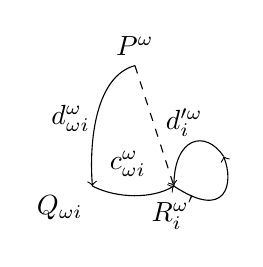
\begin{tikzpicture}[scale=.9]
\coordinate (P) at (.6,1.7);\coordinate (Q) at (0,0);\coordinate (R) at (1.15,0);
\draw[->] (P)..controls (.05,1.55) and (-.05,.65)..(Q);
\draw[dashed,->] (P)--(R);\draw[->] (Q)..controls (.35,-.18) and (.85,-.18)..(R);
\draw[->] (R)..controls (1.9,-.5) and (2,.05)..(1.85,.42);\draw (1.85,.42)..controls (1.6,.8) and (1.15,.7)..(R);
\node[above] at (P) {$P^\omega$};\node[below left] at (Q) {$Q_{\omega i}$};\node[below] at (R) {$R_i^{\omega'}$};
\node[left] at (.1,.95) {$d_{\omega i}^\omega$};\node[right] at (.9,.9) {$d_i^{\prime\omega}$};\node[above] at (.5,0) {$c_{\omega i}^\omega$};
\end{tikzpicture}}
par la formule
\margin{36}

\scanpage{38}
\mspage{\textcircled{19}}
\[
(67)\qquad u(\widetilde d_i^{\prime\omega})=\varphi_i^{\omega'}(\underbrace{\zeta'}_{\eta\zeta})\widetilde d_i^{\prime\omega}
\]
On a aussi des chemins
\diagram{\begin{tikzcd}[ampersand replacement=\&,column sep=large,row sep=large]
P^\omega\arrow[rr,"d_i^\omega"]\arrow[dr,"d_{\omega'i}^\omega"']\&\&R_i^\omega\\
\&Q_{\omega'i}\arrow[ur,"c_{\omega'i}^{\omega'}"']\&
\end{tikzcd}}\quad(66')
\[
d_i^\omega=c_{\omega'i}^{\omega'}\cdot d_{\omega'i}^\omega
\]
\margin{\diagram{\begin{tikzcd}[ampersand replacement=\&,column sep=small,row sep=large]
\&P_\infty^\omega\arrow[d,"d_{\omega'i}^\omega"]\arrow[dl,dashed]\\
R_i^\omega\&Q_{\omega'i}\arrow[l,bend left=15,"c_{\omega'i}^{\omega'}"]
\end{tikzcd}}}
\margin{NB $\tau(d_i^\omega)=d_i^{\prime\omega}$}
et on aura également
\[
(67')\qquad u(\widetilde d_i^\omega)=\varphi_i^\omega(\eta\widetilde\sigma_\infty(\zeta))\widetilde d_i^\omega
\]
\figure{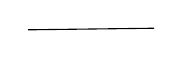
\begin{tikzpicture}\draw (0,0)--(1.6,.02);\end{tikzpicture}}

Je vois encore deux cas à regarder, savoir les sous-groupoïdes pleins de $\overline{\underline{\mathrm{VI}}}$ induits sur les \inserted{huit} sommets $(R_{i,\omega},P^\omega)$, soit $\overline{\underline{\mathrm{VII}}}$, décrit par le graphe de $=$ nom et les flèches $d_i^{\prime\omega},d_i^\omega,a_i^\omega,b_i^\omega$ (24 flèches), et celui induit sur les \deleted{cinq points} \inserted{sommets} $Q_i,P^\omega$ --- à strictement parler, c'est le groupoïde déjà nommé $\overline{\underline{\mathrm{IV}}}$ ayant les $=$s \deleted{objets} sommets, mais
\figure{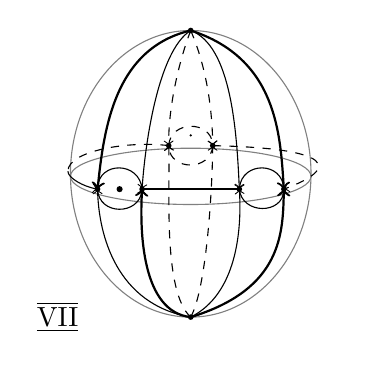
\begin{tikzpicture}[scale=.65]
\draw[gray] (0,0) ellipse (2.35 and 2.8);\draw[gray] (0,-.05) ellipse (2.35 and .55);
\coordinate (P) at (0,2.8);\coordinate (M) at (0,-2.8);
\coordinate (A) at (-1.82,-.3);\coordinate (B) at (-.95,-.3);
\coordinate (C) at (-.43,.55);\coordinate (D) at (.43,.55);
\coordinate (E) at (.95,-.3);\coordinate (F) at (1.82,-.3);
\foreach \p in {P,M,A,B,C,D,E,F}{\fill (\p) circle (.055);}
\draw[thick,->] (P)..controls (-1.5,2.45) and (-1.7,.85)..(A);
\draw[->] (P)..controls (-.65,2.4) and (-.9,.5)..(B);
\draw[dashed,->] (P)..controls (-.25,2.15) and (-.44,1.25)..(C);
\draw[dashed,->] (P)..controls (.3,2.1) and (.42,1.3)..(D);
\draw[->] (P)..controls (.8,2.5) and (.9,.8)..(E);
\draw[thick,->] (P)..controls (1.7,2.25) and (1.75,.75)..(F);
\draw[->] (M)..controls (-1.45,-2.55) and (-1.8,-1.2)..(A);
\draw[thick,->] (M)..controls (-.95,-2.7) and (-1,-1.15)..(B);
\draw[dashed,->] (M)..controls (-.55,-2.3) and (-.4,-.3)..(C);
\draw[dashed,->] (M)..controls (.3,-2.25) and (.42,-.4)..(D);
\draw[->] (M)..controls (.9,-2.35) and (1,-1.1)..(E);
\draw[thick,->] (M)..controls (1.8,-2.25) and (1.8,-1.15)..(F);
\draw[<-] (B)..controls (-1,-.82) and (-1.8,-.82)..(A);
\draw[->] (B)..controls (-1,.25) and (-1.8,.25)..(A);
\draw[dashed,->] (C)..controls (-.4,1.05) and (.4,1.05)..(D);
\draw[dashed,->] (D)..controls (.4,.05) and (-.4,.05)..(C);
\draw[<-] (E)..controls (1,.25) and (1.8,.25)..(F);
\draw[->] (E)..controls (1,-.8) and (1.8,-.8)..(F);
\draw[thick] (B)--(E);
\draw[dashed] (C)..controls (-1.2,.65) and (-2.4,.45)..(-2.4,.05);\draw[->] (-2.4,.05)..controls (-2.4,-.08) and (-2.1,-.25)..(A);
\draw[dashed,->] (D)..controls (2.85,.5) and (2.9,.1)..(F);
\fill (-1.39,-.3) circle (.06);\fill (0,.75) circle (.025);
\node at (-2.6,-2.8) {$\overline{\underline{\mathrm{VII}}}$};
\end{tikzpicture}}
\margin{\uline{NB} les $b_i^\omega$ reliant directement les $Q_i$ sont ici inutiles}
\figure{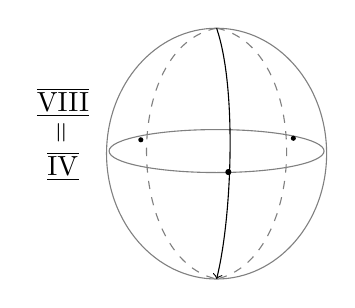
\begin{tikzpicture}[scale=.65]
\draw[gray] (0,0) ellipse (2.15 and 2.45);
\draw[gray] (0,.05) ellipse (2.1 and .42);
\draw[gray,dashed] (0,2.45)..controls (-1.85,2.1) and (-1.8,-2.05)..(0,-2.45);
\draw[gray,dashed] (0,2.45)..controls (1.85,2.1) and (1.8,-2.05)..(0,-2.45);
\draw[->] (0,2.45)..controls (.4,1.3) and (.3,-1.25)..(0,-2.45);
\fill (-1.48,.27) circle (.05);\fill (1.5,.3) circle (.05);\fill (.23,-.36) circle (.06);
\node at (-3,1) {$\overline{\underline{\mathrm{VIII}}}$};\node[rotate=90] at (-3,.4) {$=$};\node at (-3,-.25) {$\overline{\underline{\mathrm{IV}}}$};
\end{tikzpicture}}
représenté par un graphe un peu plus grand --- dans $\boxed{\mathrm{VIII}}$ on distingue les \inserted{six} \deleted{flèches} $d_i^\omega$ seulement, et on en donne pas en plus les $\widetilde a_i^\omega$, ce qui est inutile en fait par (35). (Donc il n'est pas étonnant que dans (37), \unsure{la|le} donnée de $\widetilde\alpha$, qui
\margin{37}

\scanpage{39}
\mspage{\textcircled{20}}
repère \inserted{les} $u(\widetilde a_i^\omega)$, résulte déjà de celle de $\zeta$, qui repère \inserted{les} $u(d_i^\omega)$,
\figure{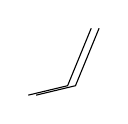
\begin{tikzpicture}[baseline=0pt]\draw (0,0)--(.5,.12)--(.8,.85);\draw (.1,0)--(.6,.12)--(.9,.85);\end{tikzpicture}}
Les graphes $\overline{\underline{\mathrm{I}}}$ à $\overline{\underline{\mathrm{VII}}}$ donnent lieu au diagramme d'inclusions
\diagram{\begin{tikzcd}[ampersand replacement=\&,column sep=2em,row sep=2.8em,execute at end picture={\draw ([xshift=-4mm,yshift=5mm]\tikzcdmatrixname-2-1.north west) rectangle ([xshift=5mm,yshift=-4mm]\tikzcdmatrixname-3-3.south east);}]
\&\&\overline{\underline{\mathrm{III}}}\arrow[dl,hook]\arrow[dr,hook]\&\&\\
\overline{\underline{\mathrm{I}}}\arrow[r,hook]\arrow[dr,hook]\&\overline{\underline{\mathrm{II}}}\arrow[dr,hook]\arrow[r,draw=none,"\deleted{\leftrightarrow}"]\&\phantom{\overline{\underline{\mathrm{II}}}}\&\overline{\underline{\mathrm{IV}}}\arrow[dl,hook]\&\mathrm{V}\arrow[l,hook]\\
\&\overline{\underline{\mathrm{VII}}}\arrow[r,hook]\&\overline{\underline{\mathrm{VI}}}\&\&
\end{tikzcd}}\quad(68)

Sans calcul, je peux déjà prédire que la donnée d'un autom. de $\overline{\underline{\mathrm{VII}}}$ fixant les sommets et commutant à $G_J$, équivaut à la donnée des quantités
\[
(69)\qquad (\uline{\lambda},\beta',\uline{\zeta'})\in\widehat\Pi_{0,3}\times\widehat\Pi_{0,3}\times\widehat\Pi_{0,3}
\]
reliés par l\deleted{\unsure{es}}' équations \deleted{(63) ici}
\[
(70)\qquad\left\{\begin{aligned}
\beta'&=\alpha'\sigma_\infty(\lambda)\\
\beta'\sigma_\infty(\beta')&=1
\end{aligned}\right.\qquad
\begin{gathered}
\text{où}\quad\alpha'=\zeta'\rho^{\deleted{\unsure{-1}}}(\zeta')^{-1}\\
\text{i.e.}\quad\alpha'\sigma_\infty(\lambda)\sigma_\infty(\alpha')\lambda=1
\end{gathered}
\]
\margin{\figure{
\begin{tikzpicture}\node[align=center] at (0,.6) {donc $\beta'$\\inutile!};\draw (-.8,.6)..controls (-.9,-.1) and (-.2,-.3)..(0,-.6)..controls (.05,-.1) and (.85,-.2)..(.9,.35);\end{tikzpicture}}}
(tout comme \inserted{dans le cas où} $\overline{\underline{\mathrm{II}}}$ est défini par \deleted{$(\lambda,\eta,\alpha')$},
\deleted{reliés par}
\[
(69')\qquad(\uline{\lambda},\uline{\eta},\alpha')\in\widehat\Pi_{0,3}\times\widehat\Pi_{0,3}\times\widehat\Pi_{0,3}
\]
avec \unsure{l'|les} équations
\[
(70')\qquad\left\{\begin{aligned}
\beta'&=\alpha'\sigma_\infty(\lambda)\\
\alpha'\rho(\alpha')\rho^2(\alpha')&=1
\end{aligned}\right.\qquad\text{où}\quad\beta'=\eta\sigma_\infty(\eta)^{-1}
\]
\margin{donc $\alpha'$ inutile!}
\margin{38}

\scanpage{40}
\mspage{21}
Je vais expliciter les calculs dans le groupoïde $\overline{\underline{\mathrm{VII}}}$, associé au graphe de $=$ nom, on a des flèches génératrices
\[
(71)\qquad\left\{\begin{aligned}
\widetilde d_i^\omega&:P^\omega\longrightarrow R_i^\omega\\
\widetilde d_i^{\prime\omega}&:P^\omega\longrightarrow R_i^{\omega'}\\
a_i^\omega&:R_i^\omega\mathbin{-}R_i^{\omega'}
\end{aligned}\right.
\]
liées par les relations
\[
(72)\qquad\left\{\begin{aligned}
(\widetilde d_i^{\omega\prime})^{-1}a_i^\omega\widetilde d_i^\omega&=1\\
(d_{\omega i}^{\prime\omega})^{-1}\widetilde d_{\omega i}^{\omega'}(d_i^{\prime\omega'})^{-1}\widetilde d_i^\omega&=1
\end{aligned}\right.
\]
\margin{six relations indépendantes exprimant les $\widetilde d_i^{\prime\omega}$ en termes des $\widetilde d_i^\omega$ et $a_i^\omega$, \inserted{ou les $a_i^\omega$ en termes des $\widetilde d_i^\omega,\widetilde d_i^{\prime\omega}$.}}
\margin{en apparence six relations, mais il n'y en a que trois indépendantes, car l'équation pour $i,\omega$ et pour $(\omega i,\omega')$ est la $=$.}
\figure{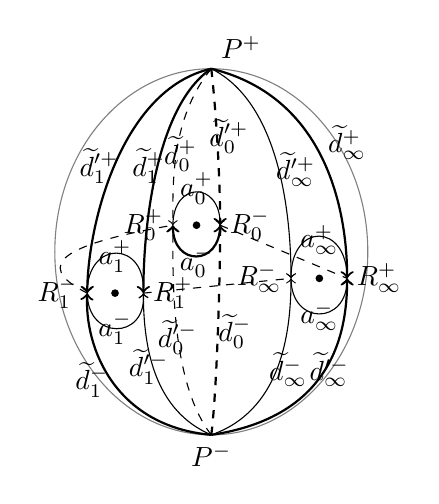
\begin{tikzpicture}[scale=.75]
\draw[gray] (0,0) ellipse (2.65 and 3.1);
\coordinate (P) at (0,3.1);\coordinate (M) at (0,-3.1);
\coordinate (L1) at (-2.1,-.7);\coordinate (R1) at (-1.15,-.7);
\coordinate (L0) at (-.65,.45);\coordinate (R0) at (.15,.45);
\coordinate (LI) at (1.35,-.45);\coordinate (RI) at (2.3,-.45);
\draw[dashed] (L1)..controls (-3.1,-.2) and (-2.4,.15)..(L0);
\draw[dashed] (R0)--(RI);\draw[dashed] (R1)--(LI);
\fill (-1.63,-.7) circle (.065);\fill (-.25,.45) circle (.065);\fill (1.83,-.45) circle (.065);
\draw[->,thick] (P)..controls (-1.55,2.75) and (-2.1,.4)..(L1);
\draw[->,thick] (P)..controls (-.9,2.5) and (-1.15,.55)..(R1);
\draw[dashed,->] (P)..controls (-.7,2.25) and (-.65,1.1)..(L0);
\draw[dashed,->,thick] (P)..controls (.1,2.2) and (.15,1.1)..(R0);
\draw[->] (P)..controls (1.2,2.5) and (1.35,.5)..(LI);
\draw[->,thick] (P)..controls (2.05,2.6) and (2.3,.5)..(RI);
\draw[->,thick] (M)..controls (-1.65,-2.95) and (-2.15,-1.6)..(L1);
\draw[->] (M)..controls (-.95,-2.7) and (-1.15,-1.65)..(R1);
\draw[dashed,->] (M)..controls (-.7,-2.2) and (-.65,-.35)..(L0);
\draw[dashed,->,thick] (M)..controls (.1,-2.3) and (.15,-.35)..(R0);
\draw[->] (M)..controls (1.15,-2.7) and (1.35,-1.45)..(LI);
\draw[->,thick] (M)..controls (2,-2.8) and (2.3,-1.45)..(RI);
\draw[->] (R1)..controls (-1.1,.2) and (-2.1,.2)..(L1);
\draw[->] (L1)..controls (-2.1,-1.5) and (-1.1,-1.5)..(R1);
\draw[->] (L0)..controls (-.65,1.2) and (.15,1.2)..(R0);
\draw[->,thick] (R0)..controls (.15,-.25) and (-.65,-.25)..(L0);
\draw[->] (RI)..controls (2.3,.5) and (1.35,.5)..(LI);
\draw[->] (LI)..controls (1.35,-1.25) and (2.3,-1.25)..(RI);
\node[above right] at (P) {$P^+$};\node[below] at (M) {$P^-$};
\node[left] at (L1) {$R_1^-$};\node[right] at (R1) {$R_1^+$};
\node[left] at (L0) {$R_0^+$};\node[right] at (R0) {$R_0^-$};
\node[left] at (LI) {$R_\infty^-$};\node[right] at (RI) {$R_\infty^+$};
\node at (-1.63,-.08) {$a_1^+$};\node at (-1.63,-1.3) {$a_1^-$};
\node at (-.25,1.07) {$a_0^+$};\node at (-.25,-.17) {$a_0^-$};
\node at (1.83,.2) {$a_\infty^+$};\node at (1.83,-1.08) {$a_\infty^-$};
\node at (-1.9,1.45) {$\widetilde d_1^{\prime+}$};\node at (-1.06,1.45) {$\widetilde d_1^+$};
\node at (-.52,1.65) {$\widetilde d_0^+$};\node at (.3,1.95) {$\widetilde d_0^{\prime+}$};
\node at (1.43,1.4) {$\widetilde d_\infty^{\prime+}$};\node at (2.3,1.85) {$\widetilde d_\infty^+$};
\node at (-2.02,-2.17) {$\widetilde d_1^-$};\node at (-1.06,-1.95) {$\widetilde d_1^{\prime-}$};
\node at (-.57,-1.45) {$\widetilde d_0^{\prime-}$};\node at (.4,-1.35) {$\widetilde d_0^-$};
\node at (1.3,-2) {$\widetilde d_\infty^-$};\node at (2,-2) {$\widetilde d_\infty^{\prime-}$};
\end{tikzpicture}}
On va repérer $u$ par les équations
\[
(73)\qquad\left\{\begin{aligned}
u(\widetilde d_i^\omega)&=\deleted{\widetilde d_i^\omega}\varphi_i^\omega(\zeta_1^{\deleted{\unsure{'}}})\widetilde d_i^\omega\\
u(\widetilde d_i^{\prime\omega})&=\deleted{\widetilde d_i^{\prime\omega}}\varphi_i^{\omega'}(\zeta')\widetilde d_i^{\prime\omega}\\
u(a_i^\omega)&=a_i^\omega\varphi_i^\omega(\lambda)
\end{aligned}\right.\qquad \zeta',\zeta_1^{\deleted{\unsure{'}}},\lambda\in\widehat\Pi_{0,3}
\]
et il reste à exprimer que $u$ satisfait les relations (72). La première s'explicite sous la forme
\[
(74)\qquad\zeta'=\varepsilon_0(\lambda\zeta_1)\qquad\text{i.e.}\quad\zeta_1=\lambda^{-1}\cdot\varepsilon_0^{-1}(\zeta')
\]
et on trouve également
\[
(75)\qquad\deleted{\beta}\zeta_1=\beta'\sigma_\infty(\zeta')
\]
\margin{où $\beta'$ défini par la condition $(65\,a))$}
Cette relations permettant de tirer $\beta'$ en termes
\margin{39}

\scanpage{41}
\mspage{22}
de $\zeta',\zeta_1$ ou de l'une de ces quantités seulement
\[
(75)\qquad\begin{aligned}
\beta'&=\zeta_1\sigma_\infty(\zeta')^{-1}=\deleted{\varepsilon_0(\lambda\zeta_1)}\zeta_1(\sigma_\infty\varepsilon_0)(\lambda\zeta_1)^{-1}\\
&=\lambda^{-1}\cdot\varepsilon_0^{-1}(\zeta')\sigma_\infty(\zeta')^{-1}.
\end{aligned}
\]
de \deleted{la dernière} \inserted{ces} expressions de $\beta'$ on tire
\[
(75')\qquad\begin{aligned}
\sigma_\infty(\beta')&=\sigma_\infty(\zeta_1)\zeta'^{-1}=\sigma_\infty(\zeta_1)\varepsilon_0(\lambda\zeta_1)^{-1}\\
&=\sigma_\infty(\lambda)^{-1}\underbrace{\overbrace{\rho(\zeta')\zeta'^{-1}}^{\alpha'^{-1}}}_{\deleted{\unsure{\alpha'}}}
\end{aligned}
\]
et la troisième expression de $\beta'$ \deleted{donne}

\deleted{$(77)$ Ce dit, l'équation que $(72\,b)$ équivaut à:}
\deleted{\[(77)\qquad\beta'\sigma_\infty(\beta')=1\]}
\deleted{soit, $\sigma_\infty(\beta')$ en posant $\beta_1=\sigma_\infty(\beta')$, pour}
\figure{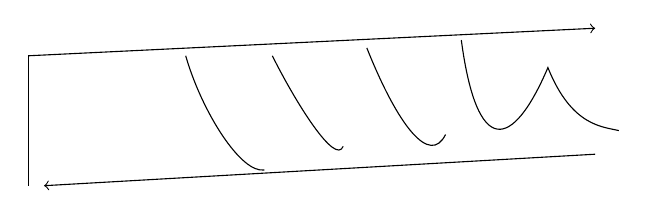
\begin{tikzpicture}[x=1cm,y=1cm]\draw[->] (0,1)--(7.2,1.35);\draw (0,1)--(0,-.65);\draw[->] (7.2,-.25)--(.2,-.65);\draw (2,1)..controls (2.2,.3) and (2.7,-.5)..(3,-.45);\draw (3.1,1)..controls (3.4,.4) and (3.9,-.4)..(4,-.15);\draw (4.3,1.1)..controls (4.7,.1) and (5.1,-.4)..(5.3,0);\draw (5.5,1.2)..controls (5.7,-.3) and (6.15,-.2)..(6.6,.85)..controls (6.9,.1) and (7.3,.1)..(7.5,.05);\end{tikzpicture}}
s'écrit aussi
\[
(77)\qquad\sigma_\infty(\beta')^{-1}=\alpha'\sigma_\infty(\lambda).
\]
Ceci posé, l'équation $(72\,b)$ équivaut à
\[
(78)\qquad\beta'\sigma_\infty(\beta')=1\qquad\text{ou encore}\quad\sigma_\infty(\beta')^{-1}=\beta'
\]
ce qui est invariant par la substitution $\beta'\mapsto\sigma_\infty(\beta')$ \unsure{ou|\deleted{dans}} $\beta'\mapsto\beta'^{-1}$, donc posant
\inserted{(sans supposer vérifiée $(*)$)}
\[
\beta_1=\sigma_\infty(\beta')^{-1}=\alpha'\sigma_\infty(\lambda)
\]
l'équation (78) équivaut à l'équation
\[
(**)\qquad\beta_1\sigma_\infty(\beta_1)=1
\]
et implique que $\beta_1=\sigma_\infty(\beta_1)^{-1}$ donc $\beta_1=\beta'$.

En résumé, on peut tout de suite poser
\[
(79)\qquad\beta'=\alpha'\sigma_\infty(\lambda)\qquad\text{où}\quad\alpha'=\zeta'\rho(\zeta')^{-1}
\]
et la relation à imposer à $(\lambda,\zeta')$ est, au choix,
\margin{40}

\scanpage{42}
\mspage{23}
l'égalité du $\beta'$ défini par cette équation avec \unsure{le|les} celui défini par \inserted{les formules équivalentes} $(75)$, ou $(75')$ ou (77), ou

\deleted{le fait que $\beta'$ \unsure{(ce|(vu}}
l'équation (78), écrite au choix pour $\beta'$ défini par l'une des formules $(75)$ à (77), ou par la formule (79) --- ce qui donne la formulation la plus simple.
\margin{41}

\scanpage{44}
\margin{43}
\mspage{1}
\margin{Attention, notations de ce qui suit p.r. à celles des calculs précédents, en $\alpha,\beta,\alpha',\beta',\zeta,\eta,\zeta'\ldots$}
Considérons une 2-sphère conforme \inserted{$\Sigma$} avec une partie $J$ à trois éléments,
\[
(1)\qquad J\subset\Sigma,\qquad J=(R_i)_{i\in J}
\]
de sorte que le groupe $G_J$ opère sur $\Sigma$ par automorphismes \deleted{orientés} directs, \deleted{et que} \deleted{$G_J\times\{1,\tau\}$ le groupe des} \inserted{tandis que le groupe des automorphismes} conformes de la situation $(\Sigma,J)$ est
\[
(2)\qquad\Gamma_{\Sigma,J}=\Gamma\simeq G_J\times\{1,\tau\}
\]
\margin{\uline{NB} L'antipodisme ne fait \uline{pas} partie de $\Gamma$, car il ne stabilise pas $J$}
$\tau$ est l'unique \deleted{anti} autom. $\ne1$ \deleted{\unsure{qui est}} qui fixe les $R_i$ \deleted{\unsure{tous}} ($\tau={}$conjugaison complexe).
\margin{donc la catégorie des $(\Sigma,J)$ équiv. à celle des couples $(J,\uline{\bar\omega})$, où $J\in(\mathrm{Ens})_3$ et $\uline{\bar\omega}\in(\mathrm{Ens})_2$ cf plus bas}
Il y a sur $\Sigma$ une unique métrique riemannienne homogène invariante pour $G_J$, \inserted{à scalaire $\lambda\in\mathbb R^{\unsure{*+|++}}$ près} \deleted{pour laquelle}, qui nous permet d'identifier canoniquement $\Sigma$ à la sphère unité dans un espace vectoriel réel euclidien $E_3$. On pose
\[
(3)\qquad\left\{\begin{aligned}
\uline{\bar\omega}&=\Omega(\Sigma)\simeq\Omega(E_3)\\
\uline{\omega}&=\Omega(J)\simeq\Omega(\Sigma_{\mathbb R})\\
\uline{\varepsilon}&=\Pi_0(\Sigma\setminus\Sigma_{\mathbb R})=\Pi_0(E\setminus V)=\Pi_0((E/V)^*)
\end{aligned}\right.
\]
\margin{ens des deux orientations de $\Sigma$, ou donc de $E$}
\margin{On pourrait écrire $E(J,\uline{\bar\omega})$ $V(J,\uline{\omega})$.}
\margin{On a
\[
\uline{\omega}\wedge\uline{\varepsilon}\wedge\uline{\bar\omega}=1
\]
i.e.
\[
(3\text{ bis})\qquad\left\{\begin{aligned}
\uline{\omega}&\simeq\uline{\varepsilon}\wedge\uline{\bar\omega}\\
\uline{\varepsilon}&\simeq\uline{\bar\omega}\wedge\uline{\omega}\\
\uline{\bar\omega}&\simeq\uline{\omega}\wedge\uline{\varepsilon}
\end{aligned}\right.
\]
par la conv. de Stokes entre orientations d'un hémisphère et celles de leur bord, plus précis (4) ici}
$V$ est le \inserted{$\mathbb R$-}sous-espace vectoriel de $E$ \uline{engendré} par les $R_J$, qui est de dimension 2, et où
\[
(4)\qquad\Sigma_{\mathbb R}=\Sigma\cap V
\]
cercle euclidien ds le plan euclidien $V$

\scanpage{45}
On aura dans $V$
\[
(4)\qquad\sum_{j\in J}R_j=0
\]
ce qui donne un isomorphisme
\[
(5)\qquad V\simeq V_J(\mathbb R)=\operatorname{Ker}(\mathbb R^J\xrightarrow[\text{somme}]{}\mathbb R)
\]
et on a, par la $3^{\text{ième}}$ formule (3)
\[
(6)\qquad\Delta=V^\perp\simeq\mathbb R(\varepsilon)
\]
\margin{``axe polair''}
\margin{orth. de $V$ dans $E$}
\margin{(isom compatible avec la structure quadratique)}
donc
\[
(7)\qquad E\simeq V_J(\mathbb R)\oplus\mathbb R(\varepsilon)
\]
\margin{isom d'espaces euclidiens}
où dans $V_J(\mathbb R)$ on prend la seule forme quadratique \inserted{$q$} pour laquelle les $R_j$ \deleted{soient} \inserted{satisfont} \deleted{de carré un}
\[
q(R_j)=1
\]
\margin{Il est clair, par cette caractérisation de $q$, que l'opération naturelle de $G_J$ sur $V(J)$ conserve $q$.}
(prenant une base formée de $R_i,R_j$, $R_n$ de coordonnées $(-1,-1)$, la forme quadratique en question est $x^2-xy+y^2$)

Dans le plan euclidien $V$, les $R_i$ \figure{\begin{tikzpicture}[baseline=0pt]\draw[->] (.3,.55)--(0,.35)--(0,0);\end{tikzpicture}} forment les sommets d'un triangle équilatéral inscrit dans le cercle unité. L'opération de $G_J$ sur $E$ se fait par son opération \deleted{sur} tautologique sur $V(J)$ et l'opération par $\operatorname{sg}(g)$ sur $\Delta$:
\margin{44}

\scanpage{46}
\mspage{2}
\[
(8)\qquad g_E=\underbrace{g_{V_J(\mathbb R)}}_{\text{tautol.}}\oplus\operatorname{sg}(g)\operatorname{id}_\Delta
\]
L'opération de $\tau$ est donnée par
\[
(9)\qquad\tau_E=\operatorname{id}_{V_J(\mathbb R)}\oplus(-\operatorname{id}_\Delta)
\]
Je pose
\[
(10)\qquad\Sigma^*=\Sigma\setminus J=\Sigma-\{R_{\deleted{\unsure{j}}\inserted{i}}\mid i\in I\}
\]
et je m'intéresse au groupoïde fondamental de $\Sigma^*$, comme exercice préliminaire de syntaxe galoisienne, avant de regarder des situations \inserted{un peu} plus complexes (le triangle équilatéral remplacé par d'autres configurations riches en symétries sur la sphère, voire sur d'autres surfaces que la sphère, ou celle-ci étant remplacée par le fibré de Hopf, en vue des applications au calcul des groupoïdes de Teichmüller...).

Il est commode d'introduire une compactification de $\Sigma^*$, pour disposer ainsi de ``pts-base'' ``proches'' desdits $R_i$.
\margin{45}

\scanpage{47}
\margin{La construction de l'éclaté marche dans le contexte des variétés $C^\infty$ et des variétés d'ailleurs analytiques réelles.}
Pour ceci, considérons l'éclaté réel de $\Sigma$ en $J$, soit $\Sigma'$, dans lequel l'image inverse de $i\in J$ s'identifie à: \deleted{$\unsure{P(}$ l'espace} la droite projective réelle
\[
(11)\qquad\Sigma'_{R_i}\simeq P(\underbrace{T_{\Sigma,R_i}})
\]
\margin{esp. tangent à $\Sigma$ en $R_i$, identifié à: $T_{\Sigma,R_i}^*/\mathbb R^*$}
qui est un cercle plongé dans la surface compacte $\Sigma'$ (qu'on peut considérer comme obtenu en enlevant de la sphère trois rondelles autour des $R_i$, et y recollant des rubans de Möbius --- on obtient une surface non \uline{orientable} dont le \deleted{genre} $\chi_!$ est égal à
\[
\begin{aligned}
&\chi_!(\Sigma)\deleted{-3}\inserted{-3\chi_!(\text{rondelle ouverte})}+3(\underbrace{\chi_!(\text{ruban Möbius})}_{0}\\
&\deleted{\unsure{\text{à}}}=2-3=-1=1-g,
\end{aligned}
\]
donc le genre est $2$).

La découpe de cette surface suivant $\bigcup\Sigma'_{R_i}$ est une surface à bord compacte, \deleted{dont} \inserted{en fait} soit $\widetilde\Sigma$, avec
\margin{$\partial\widetilde\Sigma$ un rev. double de $\coprod_i\Sigma'_{R_i}$}
\[
(12)\qquad\partial\widetilde\Sigma\simeq\coprod_{i\in I}\underbrace{TU_{\Sigma,R_i}}
\]
\margin{cercle tangent à $\Sigma$ en $R_i$, identifiable à $T_{\Sigma,R_i}^*/\mathbb R^{*+}$ noté aussi $U_i$}
\margin{$\widetilde\Sigma$ est une sphère à bord à trois trous. Notons que $\widetilde\Sigma^\circ$ a une structure conforme, mais que celle-ci ne se prolonge pas à $\widetilde\Sigma$.}
\margin{46}

\scanpage{48}
\mspage{3}
On a les équivalences de catégories
\diagram{
\begin{tikzcd}[ampersand replacement=\&]
(13)\quad \operatorname{Rev\,\text{ét}}(\widetilde\Sigma) \arrow[r,"\approx","\text{équiv}"'] \& \operatorname{Rev\,\text{et}}(\widetilde\Sigma^\circ) \arrow[r,"\sim","\text{iso}"'] \& \operatorname{Rev\,\text{et}}(\Sigma^*)
\end{tikzcd}
}
déduites de l'inclusion
\[
\widetilde\Sigma^\circ \overset{\mathrm{def}}= \widetilde\Sigma\setminus\partial\widetilde\Sigma = \widetilde\Sigma|\Sigma^* \hookrightarrow \widetilde\Sigma
\]
et de l'isomorphisme
\[
\widetilde\Sigma^\circ \xrightarrow{\sim} \Sigma^*,
\]
d'où une équivalence entre les groupoïdes fondamentaux au sens large (dt les objets sont les rev. étales 1-connexes)\deleted{des}
\[
(14)\qquad \Pi_1(\widetilde\Sigma) \longrightarrow \Pi_1(\Sigma^*)
\]
et en composant avec
\[
\Pi_1(U_i)\longrightarrow \Pi_1(\widetilde\Sigma)
\]
déduit de l'inclusion $U_i\hookrightarrow\widetilde\Sigma$, on trouve
\[
(15)\qquad \Pi_1(\deleted{\unsure{\Sigma}}U_i)\longrightarrow\Pi_1(\Sigma^*).
\]
Nous allons représenter graphiquement l'homomorphisme 14, en ``dessinant'' $\widetilde\Sigma$ sur $\Sigma^*$, comme une région qui serait contenue dans $\Sigma^*$ en lui enlevant \inserted{l'intérieur de} trois disques \inserted{fictifs} $\Delta_i$ ``infiniment petits'' \deleted{et} (s'identifiant aux disques unités des $T_{\Sigma,R_i}$ \deleted{\unsure{g}}, ou encore aux cônes sur les $U_i$), et on se représentera (14) comme provenant d'une telle inclusion fictive.
\margin{Plus précisément au lieu de travailler sur $\Sigma^*$, nous travaillons sur $C$ ``sphère à trous'' un peu plus grande que $\widetilde\Sigma$.}
\margin{47}

\scanpage{49}
En fait, nous allons travailler avec des éléments de $\Pi_1(\widetilde\Sigma)$ qui proviennent, soit de p\textsuperscript{ts} de $\widetilde\Sigma$, donc de p\textsuperscript{ts} de $\Sigma^*$ ou d'un des $U_i$, soit des \uline{parties} de $\widetilde\Sigma$ qui sont 1-connexes pour la top. induite par $\widetilde\Sigma$ -- en partant peut-être des parties \inserted{1-conn.} de $\Sigma^*$, et en les faisant ``déborder'' sur $\widetilde\Sigma$ de façon naturelle.

Le groupe $\Gamma$ opère sur la situation \inserted{$C^\infty$} $(\Sigma,J)$, donc par transport de structure sur la situation
\[
\widetilde\Sigma\longrightarrow\Sigma,\quad J\subset\Sigma
\]
donc sur \deleted{le} (14) (15). Un aspect essentiel du travail à faire est de garder \deleted{cette} constamment présente à l'esprit cette opération, et d'introduire des notations et des constructions qui soient invariantes, dans le sens requis par la situation, par les opérations en question.
\margin{48}

\scanpage{50}
\mspage{4}
\figure{
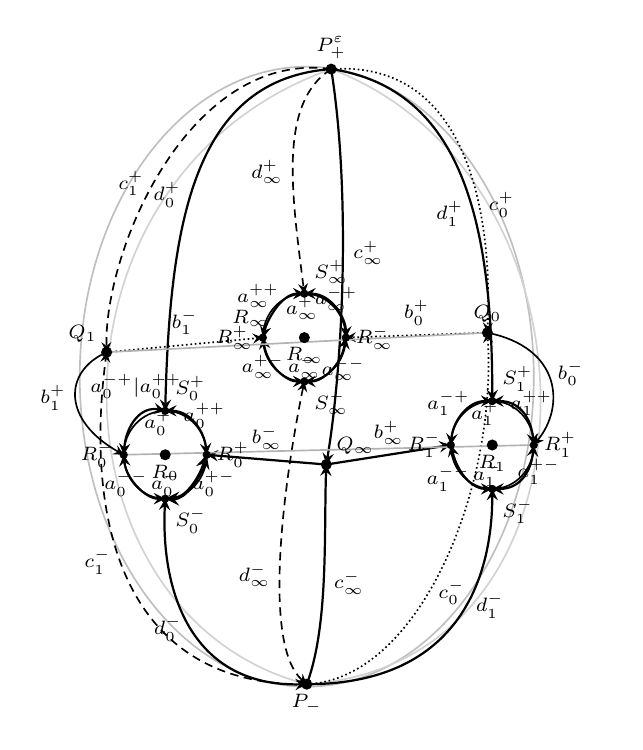
\begin{tikzpicture}[x=.62cm,y=.62cm,>=stealth,every node/.style={font=\scriptsize},line width=.6pt]
\coordinate (Pp) at (5.2,13.2); \coordinate (Pm) at (4.7,.6);
\coordinate (Qz) at (8.4,7.8); \coordinate (Qo) at (.6,7.4); \coordinate (Qi) at (5.1,5.1);
\coordinate (Rz) at (1.8,5.3); \coordinate (Ro) at (8.5,5.5); \coordinate (Ri) at (4.65,7.7);
\draw[gray!50] (4.7,6.9) ellipse (4.65 and 6.35);
\draw[gray!35] (Pp) .. controls (-1,11) and (-.7,2) .. (Pm) .. controls (11,1) and (11,11) .. (Pp);
\draw[densely dashed,->] (Pp) .. controls (2.3,13.6) and (.55,9.5) .. (Qo) node[pos=.55,left] {$c_1^+$};
\draw[densely dashed,->] (Pm) .. controls (.9,.55) and (.15,4) .. (Qo) node[pos=.55,left] {$c_1^-$};
\draw[densely dotted,->] (Pp) .. controls (8.1,13.4) and (8.5,10) .. (Qz) node[pos=.64,right] {$c_0^+$};
\draw[densely dotted,->] (Pm) .. controls (7,.7) and (8.6,4.6) .. (Qz) node[pos=.43,right] {$c_0^-$};
\draw[thick,->] (Pp) .. controls (5.6,10.7) and (5.45,7.2) .. (Qi) node[pos=.45,right] {$c_\infty^+$};
\draw[thick,->] (Pm) .. controls (5.15,1.8) and (5.05,3.7) .. (Qi) node[pos=.48,right] {$c_\infty^-$};
\draw[thick,->] (Pp) .. controls (2.4,13.0) and (1.9,10.1) .. (1.8,6.2) node[pos=.56,left] {$d_0^+$};
\draw[thick,->] (Pp) .. controls (7.9,12.8) and (8.5,10) .. (8.5,6.4) node[pos=.6,left] {$d_1^+$};
\draw[densely dashed,->] (Pp) .. controls (4.1,12.5) and (4.4,10.6) .. (4.65,8.6) node[pos=.56,left] {$d_\infty^+$};
\draw[thick,<->] (Pm) .. controls (2.4,.55) and (1.7,2.4) .. (1.8,4.4) node[pos=.5,left] {$d_0^-$};
\draw[thick,->] (Pm) .. controls (7.9,.6) and (8.5,2.9) .. (8.5,4.6) node[pos=.55,right] {$d_1^-$};
\draw[densely dashed,<->] (4.65,6.8) .. controls (4.2,4.6) and (3.8,1.4) .. (Pm) node[pos=.55,left] {$d_\infty^-$};
\draw[->,densely dotted] (Qo)--(3.8,7.7) node[midway,above] {$b_1^-$};
\draw[->,densely dotted] (Qz)--(5.5,7.7) node[midway,above] {$b_0^+$};
\draw[thick,->] (Qi)--(2.65,5.3) node[midway,above] {$b_\infty^-$};
\draw[thick,->] (Qi)--(7.65,5.5) node[midway,above] {$b_\infty^+$};
\draw[->] (Qo) .. controls (-.3,7) and (-.3,6) .. (.95,5.3) node[pos=.5,left] {$b_1^+$};
\draw[->] (Qz) .. controls (9.9,7.5) and (10,6.3) .. (9.35,5.5) node[pos=.45,right] {$b_0^-$};
\draw (Rz) ellipse (.85 and .9); \draw (Ro) ellipse (.85 and .9); \draw (Ri) ellipse (.85 and .9);
\draw[<->,thick] (1.8,6.2) .. controls (1.3,6.3) and (1,5.9) .. (.95,5.3);
\draw[<->,thick] (1.8,6.2) .. controls (2.3,6.2) and (2.6,5.8) .. (2.65,5.3);
\draw[<->,thick] (.95,5.3) .. controls (1,4.8) and (1.4,4.4) .. (1.8,4.4);
\draw[<->,very thick] (2.65,5.3) .. controls (2.5,4.8) and (2.2,4.4) .. (1.8,4.4);
\draw[<->,thick] (8.5,6.4) .. controls (8,6.4) and (7.7,6) .. (7.65,5.5);
\draw[<->,thick] (8.5,6.4) .. controls (9.1,6.4) and (9.3,6) .. (9.35,5.5);
\draw[<->,thick] (7.65,5.5) .. controls (7.8,4.9) and (8.1,4.6) .. (8.5,4.6);
\draw[<->,thick] (8.5,4.6) .. controls (9.1,4.6) and (9.3,5) .. (9.35,5.5);
\draw[<->,thick] (4.65,8.6) .. controls (4.2,8.6) and (3.9,8.1) .. (3.8,7.7);
\draw[<->,thick] (4.65,8.6) .. controls (5.2,8.6) and (5.5,8.1) .. (5.5,7.7);
\draw[<->,thick] (3.8,7.7) .. controls (3.9,7.1) and (4.3,6.8) .. (4.65,6.8);
\draw[<->,thick] (5.5,7.7) .. controls (5.4,7.1) and (5,6.8) .. (4.65,6.8);
\draw[gray!60] (Qo)--(Qz) (.95,5.3)--(9.35,5.5);
\foreach \p in {Pp,Pm,Qz,Qo,Qi,Rz,Ro,Ri} \fill (\p) circle (2pt);
\foreach \x/\y in {1.8/6.2,1.8/4.4,.95/5.3,2.65/5.3,8.5/6.4,8.5/4.6,7.65/5.5,9.35/5.5,4.65/8.6,4.65/6.8,3.8/7.7,5.5/7.7} \fill (\x,\y) circle (1.5pt);
\node[above] at (Pp) {$P_{+}^{\deleted{\unsure{\varepsilon}}}$}; \node[below] at (Pm) {$P_-$};
\node[above left] at (Qo) {$Q_1$}; \node[above] at (Qz) {$Q_0$}; \node[above right] at (Qi) {$Q_\infty$};
\node[below] at (Rz) {$R_0$}; \node[below] at (Ro) {$R_1$}; \node[below] at (Ri) {$R_\infty$};
\node[left] at (.95,5.3) {$R_0^-$}; \node[right] at (2.65,5.3) {$R_0^+$};
\node[left] at (7.65,5.5) {$R_1^-$}; \node[right] at (9.35,5.5) {$R_1^+$};
\node[left] at (3.8,7.7) {$R_\infty^+$}; \node[right] at (5.5,7.7) {$R_\infty^-$};
\node[above right] at (1.8,6.2) {$S_0^+$}; \node[below right] at (1.8,4.4) {$S_0^-$};
\node[above right] at (8.5,6.4) {$S_1^+$}; \node[below right] at (8.5,4.6) {$S_1^-$};
\node[above right] at (4.65,8.6) {$S_\infty^+$}; \node[below right] at (4.65,6.8) {$S_\infty^-$};
\node at (1.2,6.7) {$\unsure{a_0^{-+}|a_0^{++}}$}; \node at (2.6,6.1) {$a_0^{++}$};
\node at (2.8,4.7) {$\unsure{a_0^{+-}}$}; \node at (1,4.7) {$a_0^{--}$};
\node at (1.65,5.95) {$a_0^+$}; \node at (1.8,4.7) {$a_0^-$};
\node at (7.6,6.35) {$\unsure{a_1^{-+}}$}; \node at (9.3,6.35) {$a_1^{++}$};
\node at (9.45,4.95) {$\unsure{a_1^{+-}}$}; \node at (7.6,4.8) {$a_1^{--}$};
\node at (8.35,6.15) {$a_1^+$}; \node at (8.4,4.9) {$a_1^-$};
\node at (3.7,8.55) {$a_\infty^{++}$}; \node at (5.3,8.5) {$\unsure{a_\infty^{-+}}$};
\node at (5.45,7.05) {$a_\infty^{--}$}; \node at (3.8,7.1) {$\unsure{a_\infty^{+-}}$};
\node at (4.6,8.3) {$a_\infty^+$}; \node at (4.65,7.1) {$a_\infty^-$};
\node at (3.55,8.1) {$\deleted{\unsure{R_\infty}}$};
\end{tikzpicture}
}
On introduit
\[
(16)\quad\left\{\begin{array}{l}
Q_i\ (i\in J)\text{ antipodique de }R_i\ \inserted{(=-R_i)}\\
R_i^\omega\in U_i\quad(i\in J,\omega\in\uline{\omega})\\
P_\varepsilon\ \deleted{\unsure{\in}}\quad(\varepsilon\in\uline{\varepsilon}=\Pi_0(\Sigma\setminus\Sigma_{\mathbb R}))\\
S_i^\varepsilon
\end{array}\right.
\]
où $P_\varepsilon$ est défini par
\[
(17)\qquad\{P_\varepsilon\}=\Delta\cap(\Sigma-\Sigma_{\mathbb R})_\varepsilon
\]
\deleted{\unsure{des} $R_i^\omega\in U_{i\mathbb R}\unsure{\simeq\omega}$}
et $R_{i\omega}$ est défini ainsi

On a une bijection canonique
\[
(18)\qquad U_{i\mathbb R}\overset{\mathrm{def}}=\underbrace{U_i\cap T_{\Sigma_{\mathbb R},R_i}}_{TU_{\Sigma_{\mathbb R},R_i}}\simeq\omega
\]
sur \deleted{cette} variété \inserted{$\Sigma_{\mathbb R}$} de dim 1, l'une des orientations de celle-ci en les points $R_i$ (donc globalement) est en corr. biunivoque avec l'une des deux directions orientées tangentes.
\margin{
\[
(19)\quad S_i^\varepsilon\in U_i\cap T_{\Sigma_i,\unsure{i}}=TU_{\Sigma_i}\ \deleted{\unsure{de} \illegible{2} \unsure{qui|que}}
\]
où $\Sigma_i$ est le grand cercle déterminé par les $P_\varepsilon^{\deleted{\unsure{\omega}}}$ et $Q_i$; on a $TU_{\Sigma_i}\simeq\uline{\varepsilon}$. Car les deux directions tangentes à $\Sigma_i$ en $R_i$ se distinguent suivant les deux hémisphères $\in\uline{\varepsilon}=\Pi_0(\Sigma\setminus\Sigma_{\mathbb R})$.
}
\margin{\uline{NB} Il faudrait introduire $\widetilde\Sigma^{(\varepsilon)}_{\deleted{\unsure{\varepsilon}}}$ $(\varepsilon\in\uline{\varepsilon})$, les deux hémisphères sur $\widetilde\Sigma$, le choix des $S_i^\varepsilon$ est caractérisé par $S_i^\varepsilon\in\widetilde\Sigma^{(\varepsilon)}_{\deleted{\unsure{\varepsilon}}}$.}
On a fait la figure en indexant
\[
J=\{0,1,\infty\}\qquad \uline{\omega}=\{+1,-1\}
\]
et en choisissant une orientation sur le sphère, i.e.
\[
\uline{\unsure{\bar\omega|\omega}}\simeq\{+1,-1\},\quad\text{d'où }\varepsilon\simeq\{+1,-1\}.
\]
\margin{$+$ donné par la perm. circulaire $1\to2\to3$\quad $-$ par l'inverse.}
\deleted{On définit des \unsure{arcs de cercle} sur $\widetilde\Sigma$}
\deleted{\inserted{choisit des chemins}}
\deleted{liant des parties de $\widetilde\Sigma$}
\deleted{$(19)\qquad a_i^\omega,\ b_i,\ c_i^\omega$}
\deleted{On choisit dorénavant une orientation de $\Sigma$ \inserted{(pour les $b_i^\omega$)} (pour éviter des notations pléthoriques, \illegible{1})}
\margin{49}

\scanpage{51}
\margin{50}
\mspage{5}
\deleted{
\[
(20)\qquad\uline{\bar\omega}\simeq\{\pm1\}\quad\text{\inserted{si besoin} i.e. on dispose }\uline{\omega}\xrightarrow{\sim}\uline{\varepsilon}
\]
donc dorénavant on identifie l'ens $\uline{\omega}=\Omega(J)$ \inserted{$=\Omega(\Sigma_{\mathbb R})$} avec l'ens $\uline{\varepsilon}$ des deux hémisphères.
}
\margin{Il s'agit d'\uline{arcs} de \unsure{l'un des} cercles, qui sont déterminés par origine, extrémité, désignation du cercle, et sens de parcours.}
\margin{\uline{NB}
\[
\operatorname{Rep}(J)\simeq J\times\uline{\omega}
\]
\[
(i,j,k)\longmapsto(i,\omega_{i\to j\to k})
\]
le paquet $(a_i^{\omega\varepsilon})$ est un torseur sous $\Gamma=G_J\times\{1,\tau\}$\qquad(22).
}
Introduisons sur $\widetilde\Sigma$ les \deleted{\unsure{arcs}} chemins simples : (segments orientés plongés)
\[
(21)\qquad\overbrace{a_i^{\omega,\varepsilon}}^{12},\quad
\overbrace{b_i^\omega}^{6},\quad\overbrace{c_i^\varepsilon}^{6},\quad\overbrace{d_i^\varepsilon}^{6},\qquad
i\in J,\ \omega\in\uline{\omega},\ \varepsilon\in\uline{\varepsilon}
\]
chaque paquet \inserted{$b,c,d$} formant un torseur sous $G_J$

$\tau$ opérant par
\[
(22)\quad \tau a_i^{\omega,\varepsilon}=a_i^{\omega,\varepsilon'},\quad
\tau b_i^\omega=b_i^\omega,\quad \tau c_i^\varepsilon=c_i^{\varepsilon'},\quad \tau d_i^\varepsilon=d_i^{\varepsilon'}.
\]
\margin{\uline{NB} on a donc \deleted{déduit}
$g(a_i^\omega)=a_{g(i)}^{g(\omega)}$ etc.}
On a
\[
(23)\qquad a_i^{\omega\varepsilon}:S_i^\varepsilon\longrightarrow\deleted{S_i^\varepsilon}R_i^\omega\text{ sur }U_i\quad\inserted{(\text{quart de tour})}
\]
\deleted{dans le sens de l'orientation de $\Sigma$ en $R_i$}
ce qui caractérise $a_i^{\omega\varepsilon}$. \deleted{explicite le fait que}
\[
(24)\qquad b_i^\omega:Q_i\longrightarrow R_{\omega'i}^{\omega'}\text{ sur }\widetilde\Sigma_{\mathbb R}\simeq\deleted{\unsure{\Sigma_{\mathbb R}}}\inserted{\operatorname{Dec}(\Sigma_{\mathbb R},J)}\ \deleted{\text{sur les}}
\]
\deleted{(chemin d'origine sur ce cercle)}
(chemin sur $\widetilde\Sigma_{\mathbb R}$, d'origine $Q_i$, dans la direction $\omega$, jusqu'à l'extrémité \deleted{\unsure{qui est}} du segment composante de $\widetilde\Sigma_{\mathbb R}\simeq\operatorname{Dic}(\Sigma_{\mathbb R},J)$, savoir $R_{\omega'i}^{\omega'}$.
\[
(25)\qquad c_i^\omega:P^\omega\mathrel{-\!\!\!-\!\!\!-}Q_i\qquad\text{suivant un arc de grand cercle}
\]
\[
(26)\qquad d_i^\omega:P^\omega\longrightarrow S_i^\omega\qquad\text{suivant un arc de grand cercle}
\]
\margin{On pose aussi
\[
(27)\quad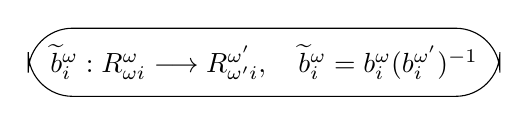
\begin{tikzpicture}[baseline=(f.base)]
\node[draw,rounded corners=16pt,inner xsep=8pt,inner ysep=6pt] (f) {$\widetilde b_i^\omega:R_{\omega i}^{\omega}\longrightarrow R_{\omega'i}^{\omega'},\quad\widetilde b_i^\omega=b_i^\omega(b_i^{\omega'})^{-1}$};
\end{tikzpicture}
\]
chemins dans la direction $\omega$ et non pour $b_i$\deleted{\unsure{des points}}\deleted{\illegible{3}}
}
Tous les arcs $\widetilde b_i^\omega,c_i^\omega,d_i^\omega$ se font sur des grands cercles de $\Sigma$, sauf que les extrémités, des $c_i^\omega,d_i^\omega$ ne sont pas dans $\Sigma^*$ mais dans \inserted{$U_i\subset$} $\partial\widetilde\Sigma\setminus\Sigma^*$
